% Options for packages loaded elsewhere
\PassOptionsToPackage{unicode}{hyperref}
\PassOptionsToPackage{hyphens}{url}
%
\documentclass[
]{book}
\usepackage{lmodern}
\usepackage{amssymb,amsmath}
\usepackage{ifxetex,ifluatex}
\ifnum 0\ifxetex 1\fi\ifluatex 1\fi=0 % if pdftex
  \usepackage[T1]{fontenc}
  \usepackage[utf8]{inputenc}
  \usepackage{textcomp} % provide euro and other symbols
\else % if luatex or xetex
  \usepackage{unicode-math}
  \defaultfontfeatures{Scale=MatchLowercase}
  \defaultfontfeatures[\rmfamily]{Ligatures=TeX,Scale=1}
\fi
% Use upquote if available, for straight quotes in verbatim environments
\IfFileExists{upquote.sty}{\usepackage{upquote}}{}
\IfFileExists{microtype.sty}{% use microtype if available
  \usepackage[]{microtype}
  \UseMicrotypeSet[protrusion]{basicmath} % disable protrusion for tt fonts
}{}
\makeatletter
\@ifundefined{KOMAClassName}{% if non-KOMA class
  \IfFileExists{parskip.sty}{%
    \usepackage{parskip}
  }{% else
    \setlength{\parindent}{0pt}
    \setlength{\parskip}{6pt plus 2pt minus 1pt}}
}{% if KOMA class
  \KOMAoptions{parskip=half}}
\makeatother
\usepackage{xcolor}
\IfFileExists{xurl.sty}{\usepackage{xurl}}{} % add URL line breaks if available
\IfFileExists{bookmark.sty}{\usepackage{bookmark}}{\usepackage{hyperref}}
\hypersetup{
  pdftitle={Resources on Presenting Results},
  pdfauthor={RMS},
  hidelinks,
  pdfcreator={LaTeX via pandoc}}
\urlstyle{same} % disable monospaced font for URLs
\usepackage{longtable,booktabs}
% Correct order of tables after \paragraph or \subparagraph
\usepackage{etoolbox}
\makeatletter
\patchcmd\longtable{\par}{\if@noskipsec\mbox{}\fi\par}{}{}
\makeatother
% Allow footnotes in longtable head/foot
\IfFileExists{footnotehyper.sty}{\usepackage{footnotehyper}}{\usepackage{footnote}}
\makesavenoteenv{longtable}
\usepackage{graphicx,grffile}
\makeatletter
\def\maxwidth{\ifdim\Gin@nat@width>\linewidth\linewidth\else\Gin@nat@width\fi}
\def\maxheight{\ifdim\Gin@nat@height>\textheight\textheight\else\Gin@nat@height\fi}
\makeatother
% Scale images if necessary, so that they will not overflow the page
% margins by default, and it is still possible to overwrite the defaults
% using explicit options in \includegraphics[width, height, ...]{}
\setkeys{Gin}{width=\maxwidth,height=\maxheight,keepaspectratio}
% Set default figure placement to htbp
\makeatletter
\def\fps@figure{htbp}
\makeatother
\setlength{\emergencystretch}{3em} % prevent overfull lines
\providecommand{\tightlist}{%
  \setlength{\itemsep}{0pt}\setlength{\parskip}{0pt}}
\setcounter{secnumdepth}{5}
\usepackage{booktabs}
\usepackage{amsthm}
\makeatletter
\def\thm@space@setup{%
  \thm@preskip=8pt plus 2pt minus 4pt
  \thm@postskip=\thm@preskip
}
\makeatother
\usepackage[]{natbib}
\bibliographystyle{apalike}

\title{Resources on Presenting Results}
\author{RMS}
\date{2021-03-12}

\begin{document}
\maketitle

{
\setcounter{tocdepth}{1}
\tableofcontents
}
\hypertarget{introduction}{%
\chapter{Introduction}\label{introduction}}

This page is an introduction. I will write some text later

\hypertarget{contents}{%
\section{Contents}\label{contents}}

\protect\hyperlink{story}{Presenting results as story telling}
Coming soon

\protect\hyperlink{tablegraph1}{Presenting results as tables and graphs 1}
Overview of general issues to consider for visual presentation of results

\protect\hyperlink{factor}{Presenting results as tables and graphs 2 factorial expts}
How to deal with multiple factors, and interactions

\protect\hyperlink{precision}{Presenting results as tables and graphs 3 Precision}
Coming soon

\protect\hyperlink{farmers}{Presenting results as tables and graphs 4 for farmers}
(Video Only)

\protect\hyperlink{papers}{Presenting in papers}
Coming soon

\protect\hyperlink{posters}{Presenting on posters}
presenting results for posters

\protect\hyperlink{audience}{Adapting to audiences}
Modifying your presentation for different audiences

\protect\hyperlink{showandtell}{Presenting as show and tell}
Coming soon

\protect\hyperlink{review}{Reviewing, critiquing and improving presentation}
Coming soon

\hypertarget{story}{%
\chapter{Presenting results as story telling}\label{story}}

\hypertarget{under-construction}{%
\section{UNDER CONSTRUCTION}\label{under-construction}}

\hypertarget{tablegraph1}{%
\chapter{Presenting results as tables and graphs 1}\label{tablegraph1}}

\hypertarget{draft}{%
\section{DRAFT}\label{draft}}

\hypertarget{video-under-construction}{%
\section{Video Under Construction}\label{video-under-construction}}

\hypertarget{the-importance-of-visualising-data}{%
\section{The importance of visualising data}\label{the-importance-of-visualising-data}}

Visualizing data is an essential part of communicating messages and results to any form of audience. An ineffective visualisation of data can communicate a very misleading message.

Building skills in data visualisation can help you to understand and see important results in other people's tables, graphs, and maps. This is in addition to enabling you to create informative visualisations of your own.

The aim of this chapter is to provide some principles behind making good data visualisations.

This guide is intended for anyone who wishes to develop their data visualisation and reporting skills. The advice presented here will be applicable to a wide variety of situations and is not specific to certain topics. Additionally, we hope that users of all ability levels will be able to take this advice to mind in their future projects and their everyday interactions with data.

{[}add some more points here - bullet pointed??{]}

\hypertarget{principles-of-data-visualisation}{%
\section{Principles of data visualisation}\label{principles-of-data-visualisation}}

Through developing your data visualisation skills, you can generate a wide variety of graphical/cartographic/tabular representations of data. This could be anything from simple bar graphs and line graphs to complicated cartograms. However, regardless of the complexity of your chosen data visualisation technique, there are certain principles that should always be followed:

\hypertarget{effectiveness}{%
\subsection{Effectiveness}\label{effectiveness}}

By effectiveness, we mean you should be ensuring that you are using the right type of visualisation for your objectives and priorities. This is the first crucial step in making sure what you produce is effective at displaying the message you intend to show. If you pick the wrong method, your visualisation will not be effective regardless of its quality.

Maps are of course for displaying data which have some form of geographic component.

Tables are suited for presenting structured numerical information; consider tables of means across some groups, frequencies, or some statistical information. This makes them ideal for when the message is in the specific numbers and potentially the relationship between them.
Graphs are quite multi-purpose; there is a type of graph for almost any message you could be wanting to convey. In general, we would choose to use them for indicating trends, making broad comparisons, or showing relationships.

For instance, the pie chart below is completely unnecessary. While it is looks fine, the information is not being shown well by the use of a graph, certainly not by a pie chart. This is not helped by there being far too many colours and countries. The more effective way to display this information would be a table.

\begin{figure}
\centering
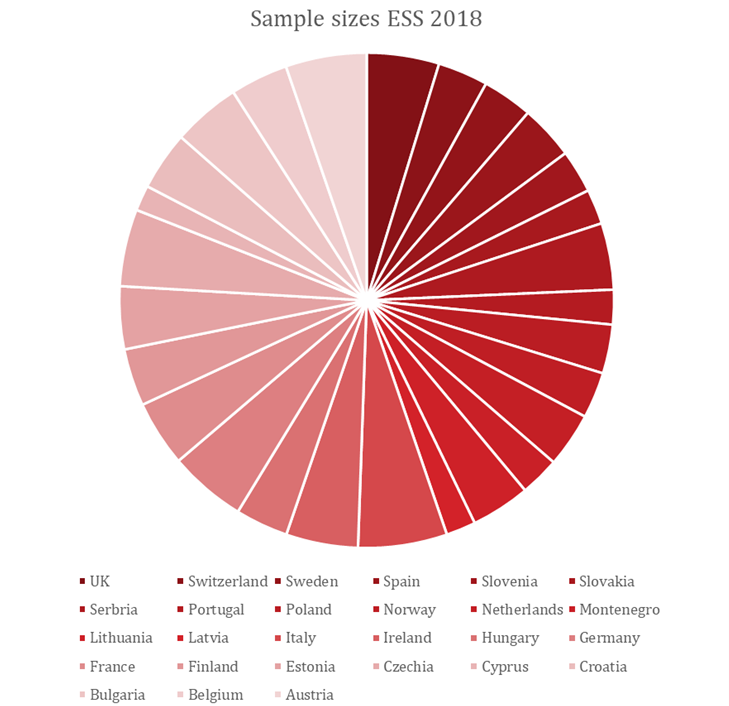
\includegraphics{img/Bad pie chart.png}
\caption{An Unnecessary Pie Chart}
\end{figure}

\hypertarget{readability}{%
\subsection{Readability}\label{readability}}

All elements of your visualisation should be legible, understandable, and coherent. In a word, readable. While this largely relates to any textual elements of your visualisations, the principle is applicable to the whole visualisation.

This includes having titles and headings which concisely explain the content. It should be informative without being overly long and confusing. The same goes for any further labels such as axis labels for graphs, column headings for tables and geographic labels on a map.

Details to consider mentioning include measurement units, geographical coverage, time, the source of the data and any relevant statistics.
Of course, the elements of a visualisation will vary depending on what visual you produce, but they should always be easy to read and understand.

You can achieve this by avoiding language beyond the scope of your target audience, providing the necessary information needed to read your visual and presenting the element in a simple and tidy manner. You will find further guidance on specific elements in each of the subsequent sections of this guide.

The example below makes a simple error. In an attempt to stop overlapping axis labels, the text size has been reduced to be far too small. A much simpler solution would have been to swap the x and y axis over. We are also missing a title and the y axis is uninformative.

\begin{figure}
\centering
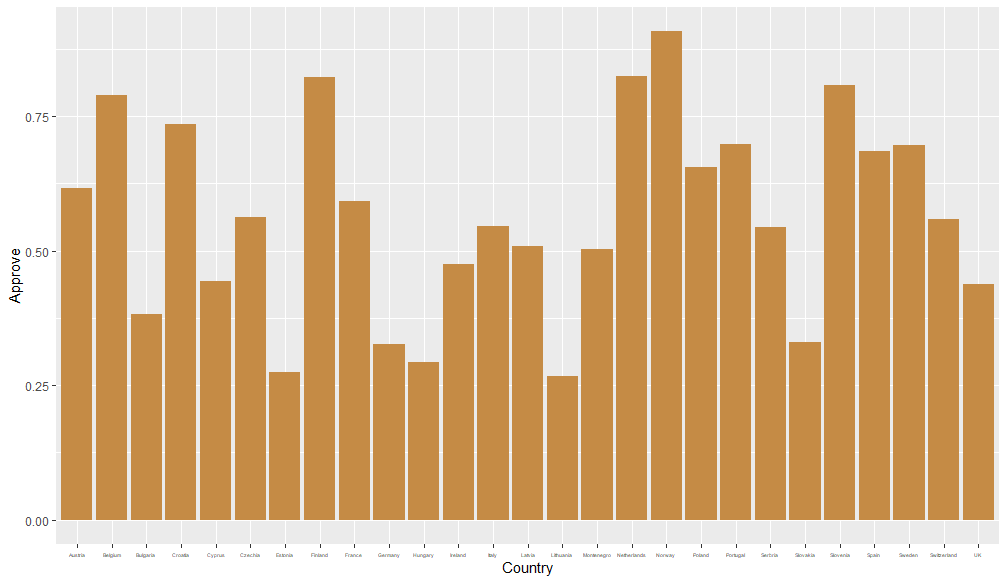
\includegraphics{img/bar chart poor.png}
\caption{Too small to read the labels}
\end{figure}

\begin{figure}
\centering
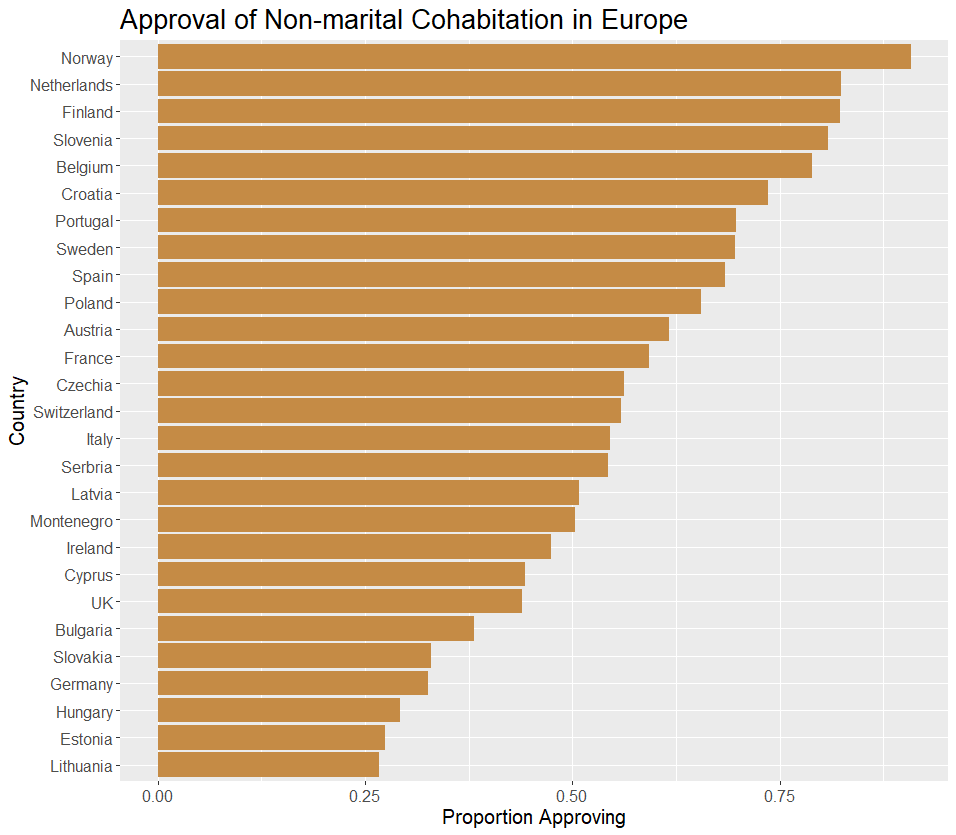
\includegraphics{img/order restored.png}
\caption{Much easier to read}
\end{figure}

\hypertarget{tidiness}{%
\subsection{Tidiness}\label{tidiness}}

A visualisation should never be cluttered. This follows on from readability, although more specifically relates to positioning and spacing of elements as well as avoiding using unnecessary elements.

This includes making sure no elements are overlapping; there should be adequate spacing between them without there being so much that it makes the visualisation look empty. This can also be described as making good use of ``white space''.

There is much more to be said on this topic, but these are mostly specific to the type of visualisation you are using. The general principle of ensuring your visual is neat and organised is always applicable.

\hypertarget{informative}{%
\subsection{Informative}\label{informative}}

A good data visualisation serves to succinctly show a message about our findings. We aim to inform our reader. Usually, it would be accompanied by some text which helps to interpret the visualisation, placing it into a wider context or providing more formal details such as the results of a relevant statistical analysis.

However, a good data visualisation should be self-explanatory and should be able to serve as a stand-alone piece. The reader should be able to understand the message without constantly referring to the text. Much of this can be accomplished by sticking to the particulars of keeping your visual tidy and readable.

Whenever creating a table, graph, or a map, you should include the source of the information from which the visualisation was created. This aids the credibility of your visualisation but also ensures a properly informed audience. An exception is when all information that is used for visualisations in a report comes from the same source. In this case, you should clearly indicate the source in advance of your visualisations.

This also means making sure that your visual is necessary in the first place. Consider the following: Can you achieve the same message with some simple text? Can a visualisation accurately demonstrate your results, or would it be distracting? Are your results too complex to visualise in isolation?

The example below makes an easy mistake in which by trying to provide too much information the plot actually becomes very difficult to read and therefore fairly uninformative as its difficult to learn anything from it. It is far too tasking to look at so many relationships at once so nothing is learned from this. Plus there are some difficult concepts being used with no understanding of measurement so this graph would not make sense out of context.

\begin{figure}
\centering
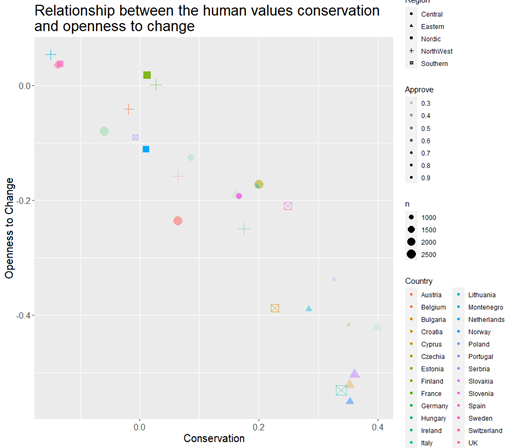
\includegraphics{img/Too many variables.png}
\caption{Far too many variables}
\end{figure}

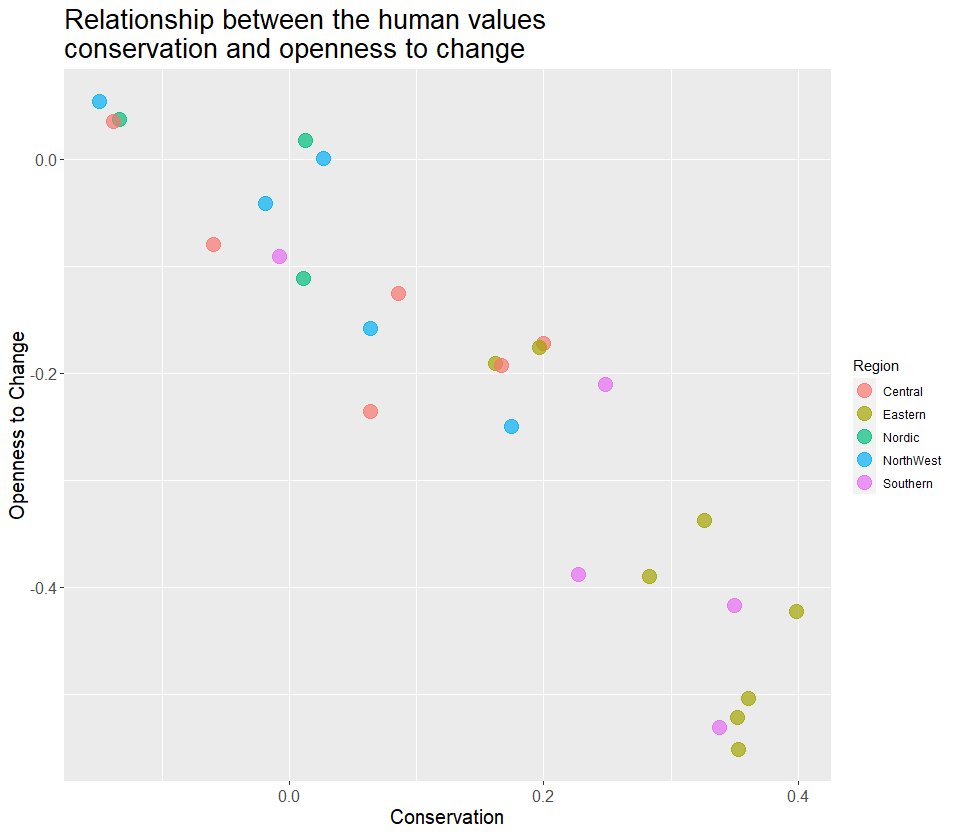
\includegraphics[width=13.28in]{img/not too much man}

Much better

\hypertarget{accessibility}{%
\subsection{Accessibility}\label{accessibility}}

Accessibility has become an increasingly important aspect of data presentation in recent years. Ensuring good practice in accessibility will help in getting an even wider audience to see our research and use our results. The Government Statistical Service makes content accessible to those with impairments to their vision, hearing, mobility, and thinking/understanding skills. For our purposes, we are mostly concerned with visual impairments.

There are some general principles on accessibility, including making sure you explain any uncommon abbreviations, avoiding clutter and keeping information concise. However, we are focusing on the use of colour. Further guidance on this is included in the accessibility section of this document. This includes considerations of colour blindness, cultural context, and the use of saturation/hue/luminance.

It is quite easy to forget to consider how our visualisations may appear to other people. The example below shows you just how different your visualisation may look to someone who suffers from visual impairments such as colour blindness.

\begin{figure}
\centering
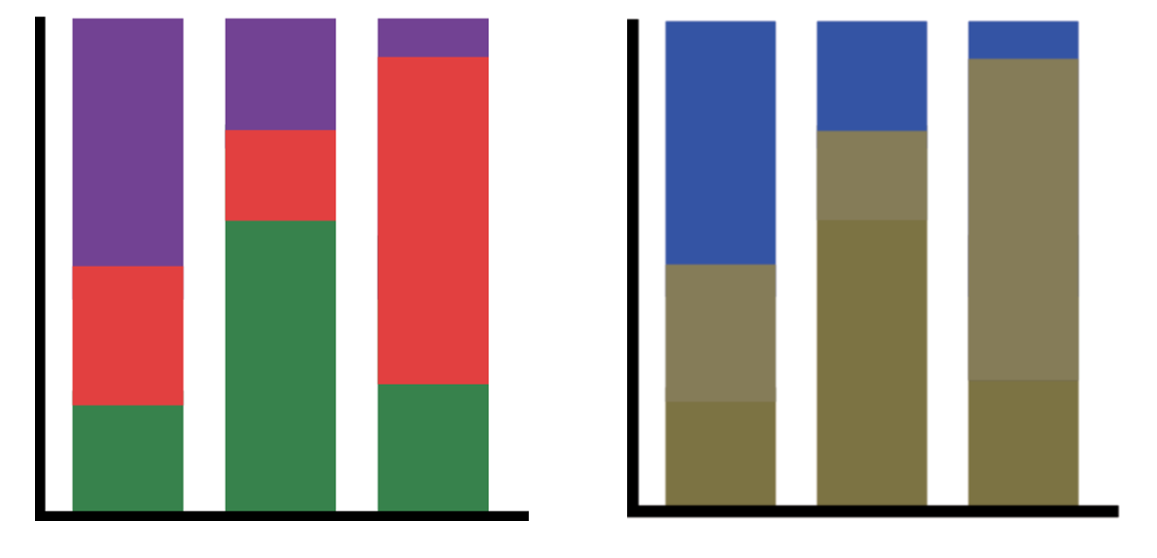
\includegraphics{img/colour blind comine.png}
\caption{Left - a normal looking graph, Right - What it looks like to a colour blind person}
\end{figure}

\hypertarget{consistency}{%
\subsection{Consistency}\label{consistency}}

This is mostly relevant when you are intending to use multiple visualisations across your report. When doing so, it is important to ensure you maintain a level of internal consistency.

This involves many aspects. For instance, if you intend to disaggregate your visuals by the levels of a variable, pay attention to the order you put these categories in. They should be kept to a logical or ascending/descending order and this order should be kept the same for the sake of consistency and readability.

The same goes for when using colours to indicate certain characteristics of the data; keep the meaning of the colours consistent.

Of course, this is also important for all the smaller details such as the font, size and face (bold/italic) of text. In essence, try to keep the formatting between visualisations as similar as possible. Generate your personal visual style and stick to it. Changing things up too much will just confuse your audience and reduce your visual's readability.

The example below unnecessary changes the order of the y axis and changes the meanning of the colours. While the graphs are okay as stand alone pieces, together they diminish the effectiveness of the whole visualisation.

\begin{figure}
\centering
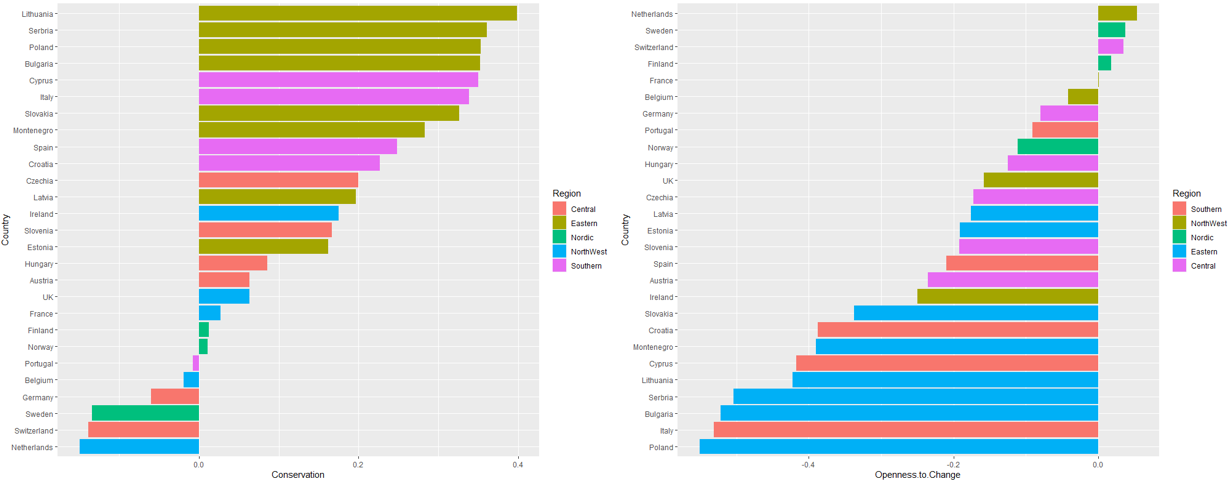
\includegraphics{img/b2b plots.png}
\caption{Unnecessary change of colour}
\end{figure}

\hypertarget{other-resources}{%
\section{Other Resources}\label{other-resources}}

\textbf{\emph{General}}

\href{}{Our extensive guide which also covers maps}

\href{https://gss.civilservice.gov.uk/policy-store/introduction-to-data-visualisation/\#section-7}{GSS -- Introduction to Data visualisation}

\href{https://stats4sd.org/resources/412}{Informative Presentation of Tables, Graphs and Statistics}

\href{https://stats4sd.org/resources/59}{Data visualisation examples}

\href{https://www.editage.com/insights/tips-on-effective-use-of-tables-and-figures-in-research-papers}{Tips on effective use of tables and figures in research papers}

\href{https://sites.google.com/site/tufteondesign/home/six-fundamental-principles-of-design}{Tufte Principles}

\href{https://blog.hubspot.com/marketing/great-data-visualization-examples}{Blog with accompanying free guide}

\textbf{\emph{Tables}}

\href{https://stats4sd.org/resources/506}{Exporting Tables from R using Flextable, Kable and gt}

\href{https://www.manuscriptedit.com/scholar-hangout/preparing-tables-research-papers/}{Preparing tables for research papers}

\href{http://www.docs.is.ed.ac.uk/skills/documents/3575/3575.pdf}{Formatting Tables in MS word}

\textbf{\emph{Graphs}}

\href{https://r-graphics.org/}{R Graphics Cookbook}

\href{https://github.com/ft-interactive/chart-doctor/blob/master/visual-vocabulary/Visual-vocabulary.pdf}{Financial Times -- Visual Vocabulary}

\textbf{\emph{Accessibility}}

\href{https://style.ons.gov.uk/writing-for-the-web/web-accessibility/introduction-3/}{ONS -- Web accessibility}

\href{https://www.tableau.com/about/blog/2016/4/examining-data-viz-rules-dont-use-red-green-together-53463}{Tableau -- Colour Blindness}

\textbf{\emph{Good Examples}}

\href{https://www.reddit.com/r/dataisbeautiful/}{Reddit - r/dataisbeautiful}

\textbf{\emph{Bad Examples}}

\href{https://www.reddit.com/r/dataisugly/}{Reddit - r/dataisugly}

\href{https://towardsdatascience.com/why-is-this-chart-bad-5f16da298afa}{towardsdatascience.com article}

\hypertarget{factor}{%
\chapter{Presenting results across multiple factors}\label{factor}}

\hypertarget{draft-1}{%
\section{DRAFT}\label{draft-1}}

\hypertarget{introduction-1}{%
\section{Introduction}\label{introduction-1}}

A common task in presenting results is how to show how an outcome variable differs across multiple explanatory factors. Often this will result from conducting a factorial treatment experiment, for example a randomised complete block design looking at whether yield varies across 5 different varieties of a crop, with 3 different levels of nitrogen fertiliser used. However the same principles are common to any analysis where we are wishing to compare the effects of multiple factors all at once, where they are designed `treatments' or observed responses from a survey.

Whenever visualising results across multiple factors we should be thinking of ways to clearly and effectively show the impacts of all of these different factors; rather than simply highlighting `best' or the 'worst.

In some cases, particularly considering a classic factorial experiment, the design of the trial itself provides a framework for how we should be visualising the results. In others there may be multiple options, some of which we can determine to be more effective than others,

\hypertarget{video}{%
\section{Video}\label{video}}

\hypertarget{overall-principles}{%
\section{Overall principles}\label{overall-principles}}

A key principle to bear in mind always is that there is never only one correct way to present results. But there definitely lots of incorrect or extremely ineffective ways. Even following a set of principles a certain amount of iteration and trial and error of different plot configurations will help the thought process and ensure that you are choosing a sensible and effective plot to convey your message. Don't expect to immediately land on the `best' answer.

What is effective depends on a few criteria:
* The message or objectives. The same data can be presented in different ways to highlight different trends.
* The design or structure of the data. Consider how many different variables you have, and how many response levels are in those variables, and what sort
* The actual observed data - this will inform scales, transformations and may lead you into presenting results in multiple different plots, or all in a single plot.
* The intended audience - a plot for publication in a journal is unlikely to be as effective if used in a presentation for a conference. And a technical audience will look for different things, and have different expectations when looking at a plot to a more general audience.

\hypertarget{example-data}{%
\section{Example Data}\label{example-data}}

The following apply to any response that is measured on experimental units, even if we usually think of a continuous variable typified by `yield'. We are going to use some simulated data in this document to show the process for comparing `yield' across a factorial experiment. The design incorporates two treatment factors - ``Type'' (A, B or C) and ``Inputs'' (0, 100 or 200). There were 20 farmers who all included the 9 treatment combinations. The 20 farmers are split across 3 sites (X, Y and Z) and we may also be interested in assessing the gender of the farmer (Male or Female).

\hypertarget{key-ideas}{%
\section{Key ideas}\label{key-ideas}}

\begin{enumerate}
\def\labelenumi{\arabic{enumi}.}
\item
  \begin{quote}
  \emph{Response to stimulus or input is observed at discrete levels of a factor}. In the example dataset we have a factorial experiment where the `response' is yield and the designed treatment factors we are considering are the combinations of `type' and `inputs'.
  We have 9 combinations or `treatments' in total: three levels of type and three levels of inputs, and 20 observations of each combination coming from the 20 farms. Therefore we have 9 mean yield values, and 9 distributions of yield, that we need to compare to be able to assess the results. Simply looking at the numbers in a table, or in a plot displayed as if these 9 treatments as independent is going to be a poor representation of the results. The numbers and plot will allow us simply to identify the highest (C/200) and lowest (b/0) treatment combinations. But it will not allow us to make any inferences easily about the overall effects of type and inputs, or the interactions between them.
  \end{quote}
\end{enumerate}

\begin{tabular}{l|r|r|r|r}
\hline
Type & Inputs & n & Mean Yield & SD Yield\\
\hline
A & 0 & 20 & 8.6 & 3.3\\
\hline
A & 100 & 20 & 10.6 & 3.6\\
\hline
A & 200 & 20 & 11.2 & 5.1\\
\hline
B & 0 & 20 & 7.7 & 3.1\\
\hline
B & 100 & 20 & 10.3 & 3.3\\
\hline
B & 200 & 20 & 10.6 & 2.7\\
\hline
C & 0 & 20 & 8.8 & 3.9\\
\hline
C & 100 & 20 & 10.4 & 4.5\\
\hline
C & 200 & 20 & 13.9 & 5.2\\
\hline
\end{tabular}

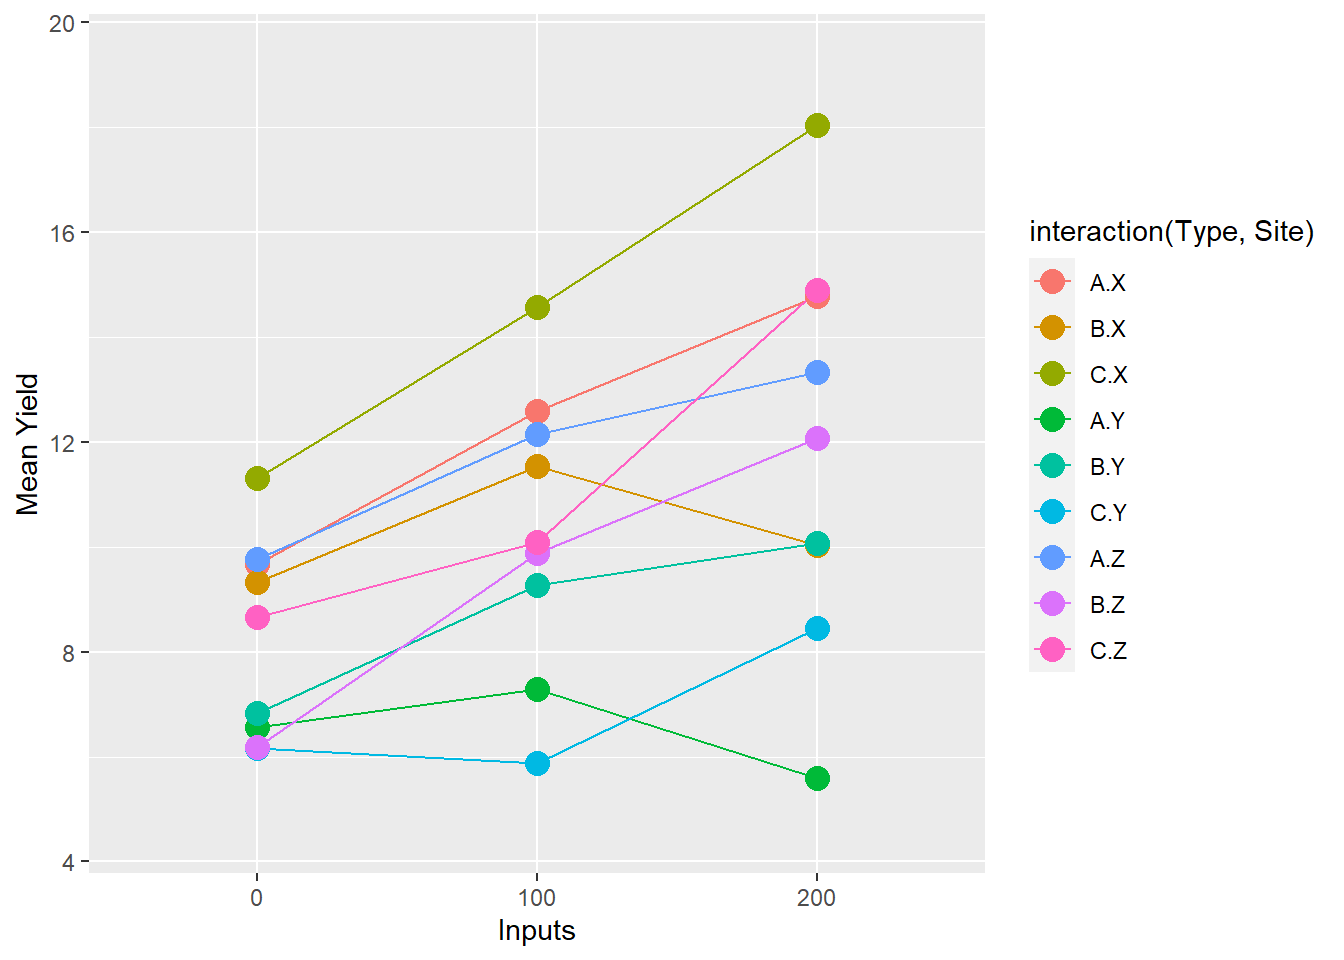
\includegraphics{PresentingResults_files/figure-latex/unnamed-chunk-8-1.pdf}

\begin{enumerate}
\def\labelenumi{\arabic{enumi}.}
\setcounter{enumi}{1}
\item
  \begin{quote}
  A conventional one-factor plot. The response on the y axis and the input or stimulus or irsk factor on the x axis.
  We could seperate out the two factors and produce seperate plots for each. This would be more informative than what we see in stage 1, since we could more easily gain an understanding of the impacts of each factor. However it would be an extremely limited interpretation by ignoring the secondary factors.
  \end{quote}
\end{enumerate}

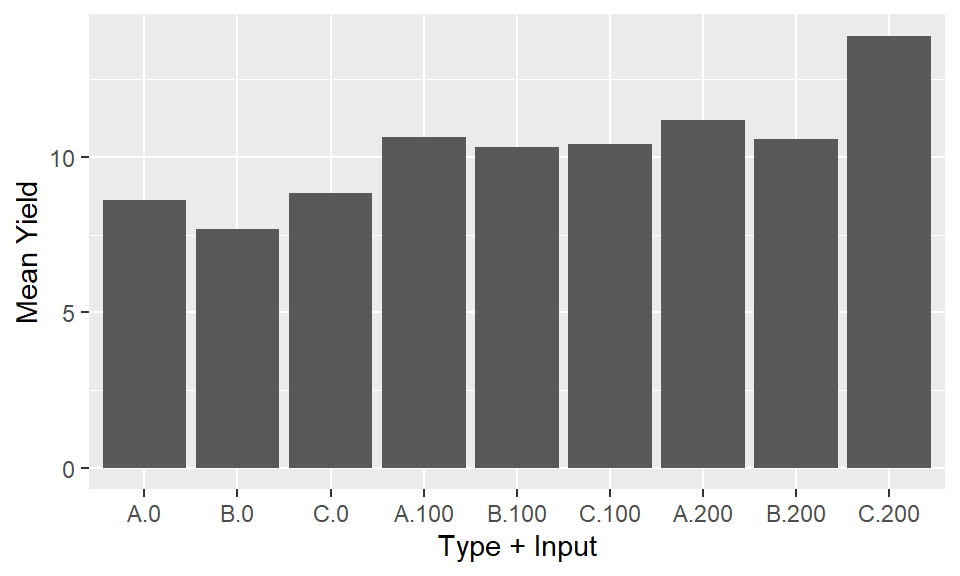
\includegraphics{PresentingResults_files/figure-latex/unnamed-chunk-9-1.pdf}

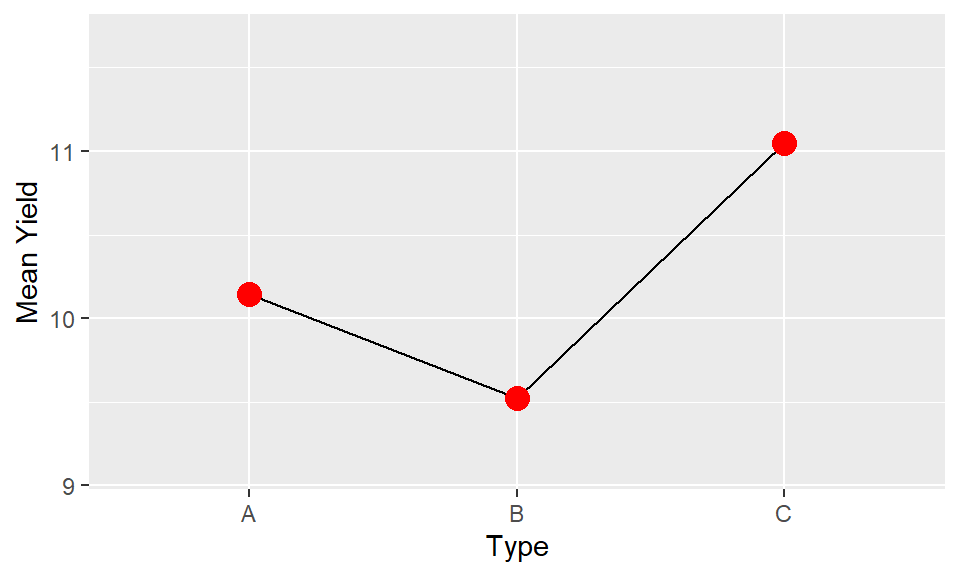
\includegraphics{PresentingResults_files/figure-latex/unnamed-chunk-10-1.pdf}

\begin{enumerate}
\def\labelenumi{\arabic{enumi}.}
\setcounter{enumi}{2}
\item
  \begin{quote}
  In most cases the interaction between factors will be of most interest. We want to understand if the impact of factor \texttt{x} and factor \texttt{y} are operating independently or if they in some way modify each other. The easiest way to understand this is through investigation of whether the trends are parallel. Parallel lines in an interaction plot suggest there is no interaction between the variables. Non-parallel lines, whether they diverge or cross, indicate there is an interaction. The ability to assess this is another reason why using lines is a much more visually powerful way to illustrate trends than using bars.
  \end{quote}
\end{enumerate}

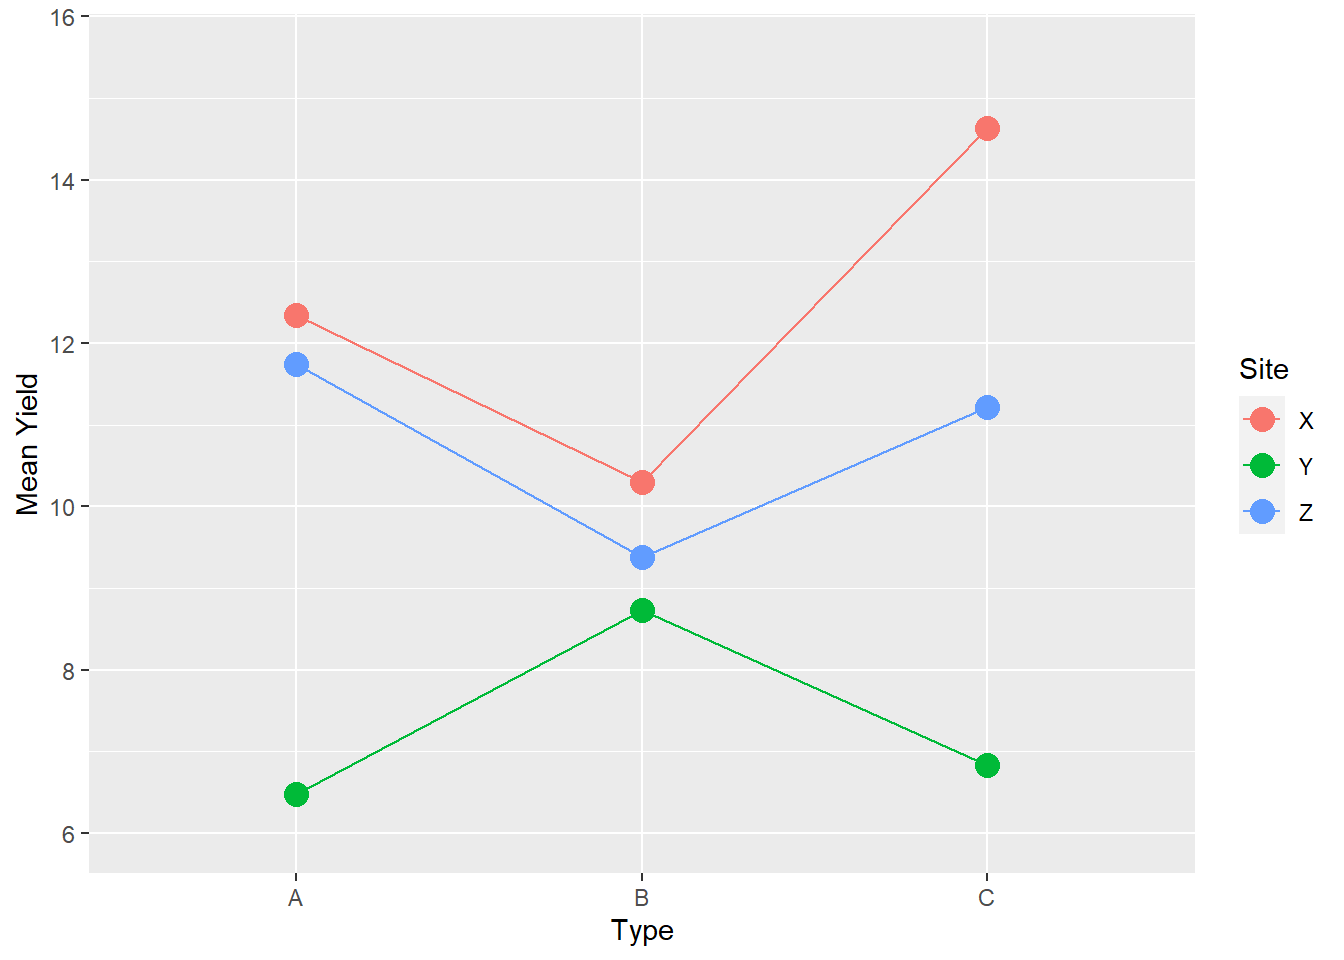
\includegraphics{PresentingResults_files/figure-latex/unnamed-chunk-11-1.pdf}

\begin{enumerate}
\def\labelenumi{\arabic{enumi}.}
\setcounter{enumi}{3}
\item
  \begin{quote}
  The interaction of ``Inputs X Type'' is the same as the interaction of ``Type X Inputs'', and the presentation provides identical information. But the way we interpret and read the plots is not the same. We may find it easier to read one particular orientation over the other. Or both orientations may be useful to highlight particular patterns which only become clearer when the positioning of the elements is reversed. It will depend on the results, and the variables themselves whether one will be more effective or whether both may be possiblities. There may not be only one way to present.
  \end{quote}
\end{enumerate}

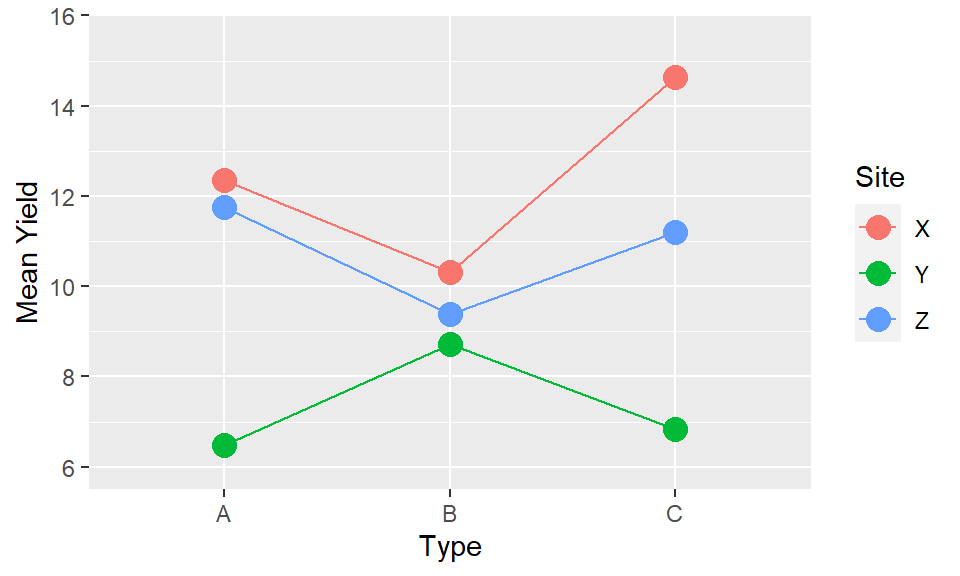
\includegraphics{PresentingResults_files/figure-latex/unnamed-chunk-12-1.pdf}

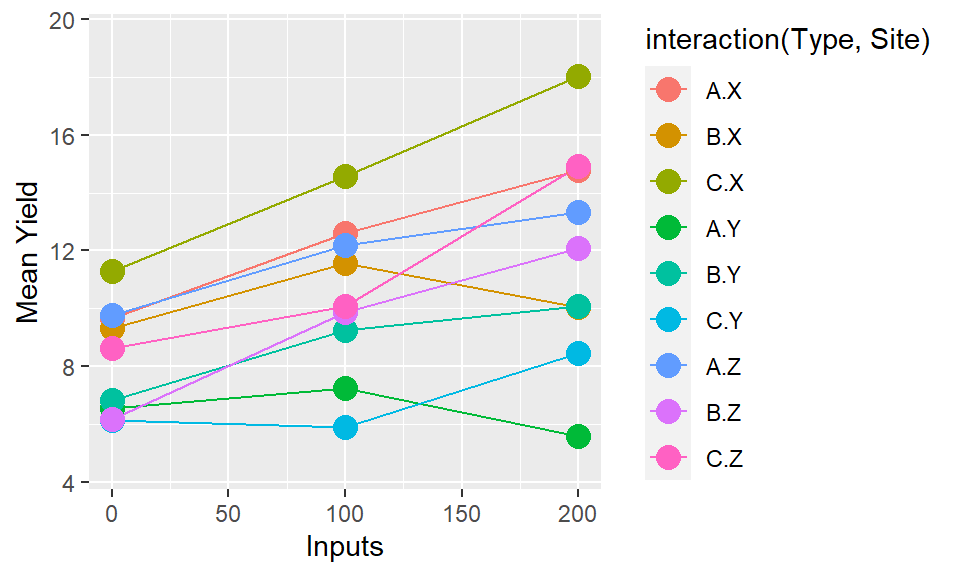
\includegraphics{PresentingResults_files/figure-latex/unnamed-chunk-13-1.pdf}

\begin{enumerate}
\def\labelenumi{\arabic{enumi}.}
\setcounter{enumi}{4}
\item
  \begin{quote}
  If there are more than two factors the same applies but more choices now and higher order interactions hard to interpret. Two choices:
  We could consider combing two factors together, if they are seen as being of equal importance, and have one line for each combination of factors. But this quickly becomes hard to interpret.
  \end{quote}
\end{enumerate}

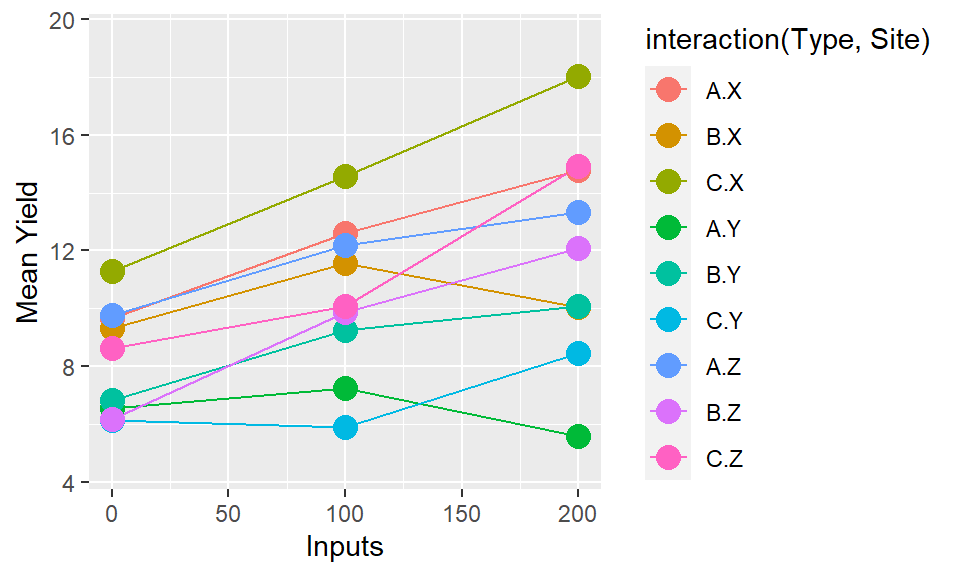
\includegraphics{PresentingResults_files/figure-latex/unnamed-chunk-14-1.pdf}

\begin{enumerate}
\def\labelenumi{\arabic{enumi}.}
\setcounter{enumi}{5}
\item
  \begin{quote}
  If there are two factors of primary interest, where the third is a modifying variable or different context, then it makes sense to use facets. In the example data we have this exact case - with Inputs and Types being our variables of primary interest, and Site being a contextual variable. Therefore plotting into multiple facets allows us to compare whether the relationships within the experiment (Input by Type) vary by the location of the experiment.
  \end{quote}
\end{enumerate}

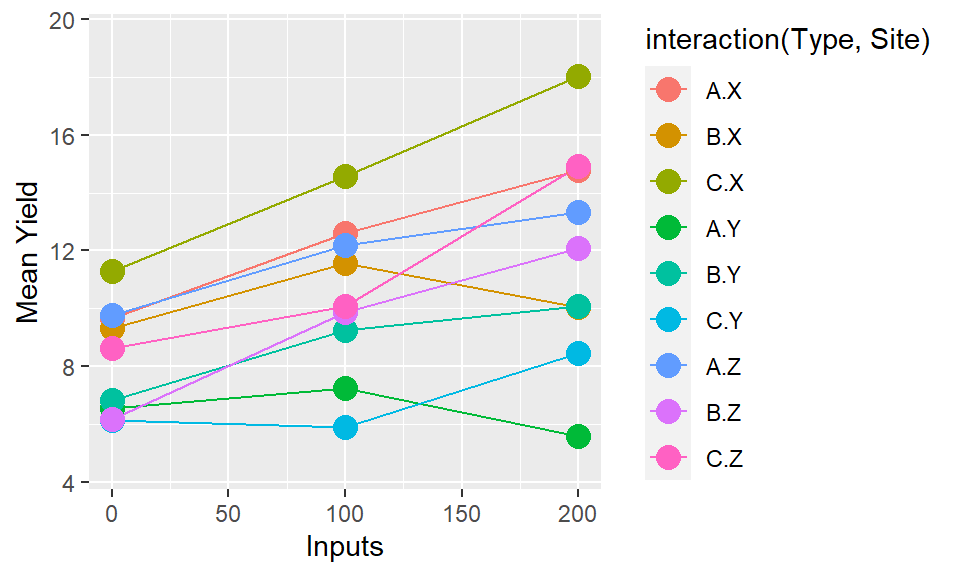
\includegraphics{PresentingResults_files/figure-latex/unnamed-chunk-15-1.pdf}

\begin{enumerate}
\def\labelenumi{\arabic{enumi}.}
\setcounter{enumi}{6}
\item
  \begin{quote}
  In practice, the observations on the graph come with uncertainty in their position. Part of the function of statistical analysis is to estimate the uncertainty so that (a) it can also be represented on the graph (b) we can separate pattern that is noise (possibly just due to random, unrepeatable variation) from that which is signal (repeatable, consistent across repetitions).
  \end{quote}
\end{enumerate}

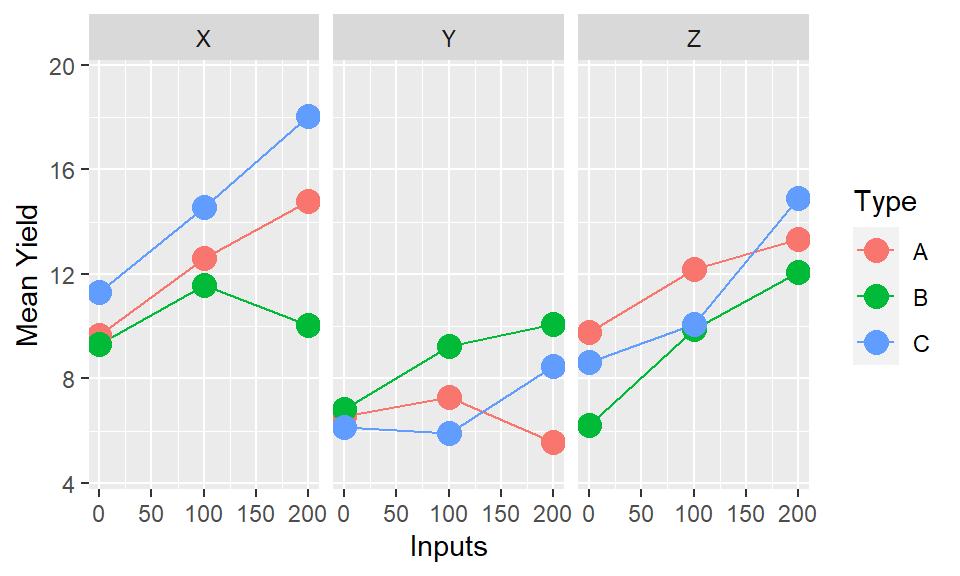
\includegraphics{PresentingResults_files/figure-latex/unnamed-chunk-16-1.pdf}

\begin{enumerate}
\def\labelenumi{\arabic{enumi}.}
\setcounter{enumi}{7}
\item
  \begin{quote}
  If the effect of one or more factors is considered noise then we can average over them and display main effects. In all of the presentations so far we have averaged over at least one of the factors to illustrate a point. But when putting the final story together we need to consider which factors are important. We should also be looking to our formal statistical analysis for guidance here, by considering which factors we have sufficient evidence to conclude are components of significant interactions. If the variables themselves are significant, but interactions are not, then averaging over these variables will be OK in terms of representing the key effects.
  \end{quote}
\end{enumerate}

\begin{verbatim}
## Type III Analysis of Variance Table with Satterthwaite's method
##                          Sum Sq Mean Sq NumDF   DenDF F value    Pr(>F)    
## Inputs                  251.632 251.632     1 130.000 50.7049 6.536e-11 ***
## Type                      9.814   4.907     2 130.000  0.9888  0.374804    
## Site                     34.314  17.157     2  19.068  3.4572  0.052346 .  
## Gender                    1.040   1.040     1  19.068  0.2095  0.652296    
## Inputs:Type              22.160  11.080     2 130.000  2.2326  0.111343    
## Inputs:Site              49.803  24.902     2 130.000  5.0178  0.007958 ** 
## Type:Site                57.372  14.343     4 130.000  2.8902  0.024828 *  
## Inputs:Gender             0.232   0.232     1 130.000  0.0467  0.829242    
## Type:Gender              13.131   6.566     2 130.000  1.3230  0.269891    
## Site:Gender              20.350  10.175     2  19.068  2.0503  0.156131    
## Inputs:Type:Site         71.161  17.790     4 130.000  3.5848  0.008297 ** 
## Inputs:Type:Gender        4.941   2.470     2 130.000  0.4978  0.609017    
## Inputs:Site:Gender       16.643   8.321     2 130.000  1.6768  0.190987    
## Type:Site:Gender         19.253   4.813     4 130.000  0.9699  0.426402    
## Inputs:Type:Site:Gender   8.019   2.005     4 130.000  0.4040  0.805502    
## ---
## Signif. codes:  0 '***' 0.001 '**' 0.01 '*' 0.05 '.' 0.1 ' ' 1
\end{verbatim}

In this case our analysis suggests Gender is not a statistically significant factor, but Inputs, Type, Site and all of the interactions between these variables are statistically significant. Therefore we should reflect that in our final plot - not showing the interactions between the three factors will be misleading, but averaging over gender will not cause any issues.

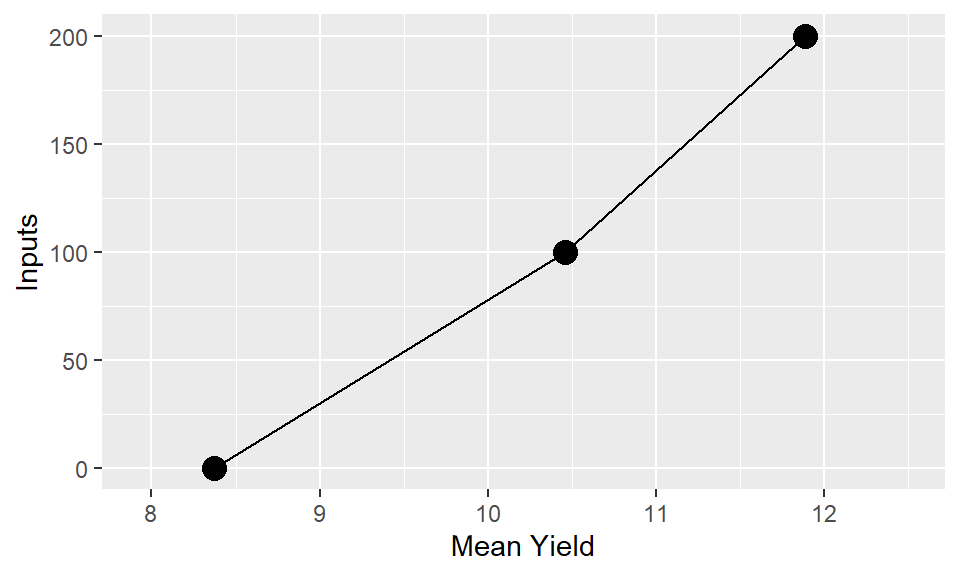
\includegraphics{PresentingResults_files/figure-latex/unnamed-chunk-18-1.pdf}

\hypertarget{shiny}{%
\section{Shiny}\label{shiny}}

\hypertarget{the-general-process}{%
\section{The general process}\label{the-general-process}}

\hypertarget{step-1-set-out-the-objectives-message-or-hypothesis-for-the-story-you-want-to-tell-with-the-graph-you-are-designing}{%
\subsection{Step 1: Set out the objectives, message or hypothesis for the story you want to tell with the graph you are designing}\label{step-1-set-out-the-objectives-message-or-hypothesis-for-the-story-you-want-to-tell-with-the-graph-you-are-designing}}

\begin{enumerate}
\def\labelenumi{\alph{enumi}.}
\item
  \begin{quote}
  There may be several messages from the same data set, so think which it is. Using the same graph for multiple purposes may sometimes be possible, but using multiple well constructed graphs will likely do a better job of illustrating these different messages.
  \end{quote}
\item
  \begin{quote}
  It does not really matter which factors are strictly treatments (randomised in the design) and which are unrandomized context factors (eg location) or observed characteristics. These maks a difference to the statistical analysis and the nature of inference, but not to the drawing of graphs.
  \end{quote}
\item
  \begin{quote}
  Likewise, complexities in layout (eg Is it split-plot design? Where there incomplete blocks? Is it a survey?) will affect the statistics, and maybe the calculation of the estimates being plotted, but not to the general design of the graphs.
  \end{quote}
\item
  \begin{quote}
  Experiments often have treatment structure that is partially or not-quite a factorial, if not all treatment combinations are present. Or there may be very poorly estimated combinations with just a few observations where the plots may be misleading if they were to be included. That's OK -- most of what is here still applies but there might be a few points that are not there or extras added. Only showing a subset of the data to focus on the specific comparisons is also a good strategy to focus the message of the plot, without the additional confusion of incomplete or very low sample size combinations.
  \end{quote}
\end{enumerate}

\begin{figure}
\centering
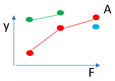
\includegraphics{img/Picture5.png}
\caption{image5}
\end{figure}

\hypertarget{step-2-remember-experiments-are-set-up-to-make-comparisons}{%
\subsection{Step 2: Remember experiments are set up to make comparisons}\label{step-2-remember-experiments-are-set-up-to-make-comparisons}}

\begin{enumerate}
\def\labelenumi{\alph{enumi}.}
\item
  \begin{quote}
  Generally the absolute value of y is less important than differences. ``Average'' rarely exists in reality, farmers are unlikely to obtain the average value of yield, but a comparison of efficacy (``A will likely yield better than B'') is more generalisable and more applicable.
  \end{quote}
\end{enumerate}

\hypertarget{step-3-maintain-the-visual-metaphor}{%
\subsection{Step 3: Maintain the visual metaphor}\label{step-3-maintain-the-visual-metaphor}}

\begin{enumerate}
\def\labelenumi{\alph{enumi}.}
\item
  \begin{quote}
  One core rule of all graphics, we want to make the way the plot is read intuitive and make sure the audience needs to refer to the axes as little as possible to understand what is being displayed. So we break the rule of response on the vertical axis with something like this:
  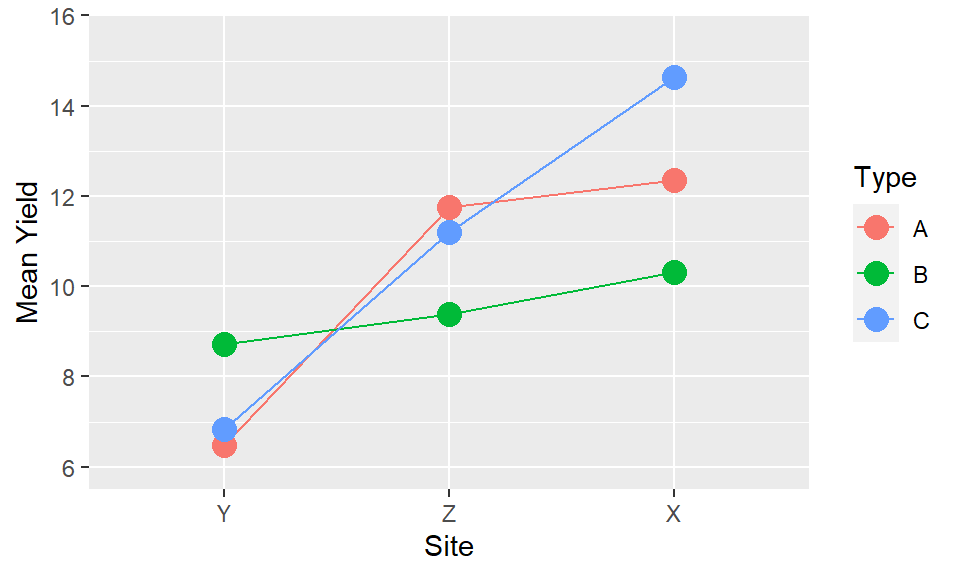
\includegraphics{PresentingResults_files/figure-latex/unnamed-chunk-20-1.pdf}
  \end{quote}
\item
  \begin{quote}
  If the horizontal axis is quantitative then the order is natural. If it is qualitative try to find an ordering that adds some value eg -- order by level of another variable, by some property of the category. Definitely do not just keep the data order, which is likely to be nothing more than purely alphabetical. In the example data we saw earlier re-ordering the sites to go from lowest to highest average yields will provide a much easier and clearer interpretation than the arbitrary alphabetical order.
  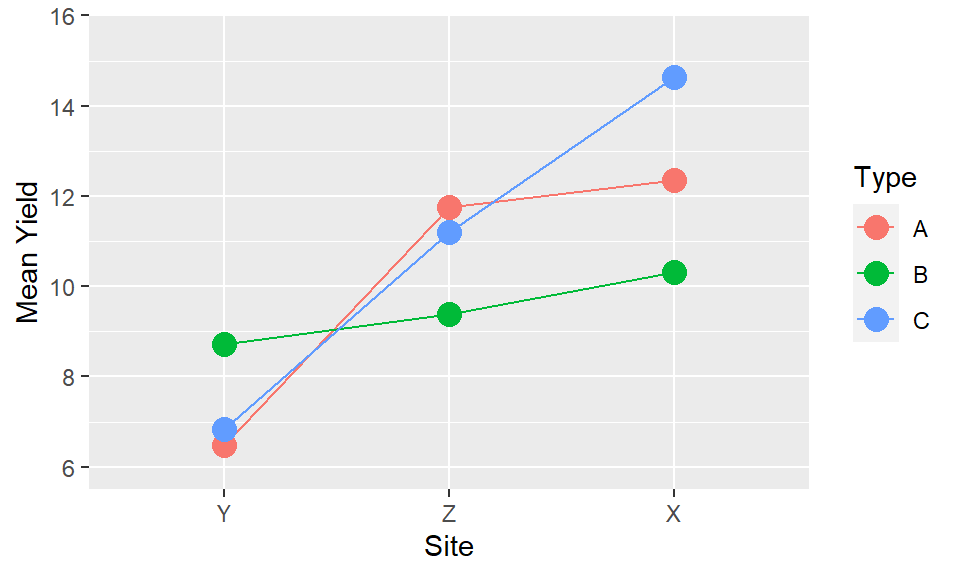
\includegraphics{PresentingResults_files/figure-latex/unnamed-chunk-21-1.pdf}
  \end{quote}
\end{enumerate}

\hypertarget{step-4-lines}{%
\subsection{Step 4: Lines}\label{step-4-lines}}

\begin{enumerate}
\def\labelenumi{\alph{enumi}.}
\item
  \begin{quote}
  Even where levels of the factor are discrete joining points together shows up which points are logically connected and the concept of interaction = non-parallel become visual. Bars are an extremely poor choice of visualisation tool for showing means, variability and comparisons across multiple factors. There use should be limited solely to percentages and frequencies, and even then only when there is a single factor being displayed.
  \end{quote}
\end{enumerate}

\hypertarget{step-5-multiple-factors}{%
\subsection{Step 5: Multiple factors}\label{step-5-multiple-factors}}

\begin{enumerate}
\def\labelenumi{\alph{enumi}.}
\item
  \begin{quote}
  More than factors is actually common, even if there are only two `treatments' when you consider location, year are often there. It would be natural to have an aim of looking at the what response to F is modified by A and whether that is the same each season (S) and local (L)
  \end{quote}
\end{enumerate}

\hypertarget{step-6-colours-and-symbols}{%
\subsection{Step 6: Colours and symbols}\label{step-6-colours-and-symbols}}

\begin{enumerate}
\def\labelenumi{\alph{enumi}.}
\item
  \begin{quote}
  Remember you can vary colour, symbol, line style. So if we do choose to plot three factors, with two factors combining to form the lines, a better option would be to have the two factors represented through different aesthetic elements.
  \end{quote}
\end{enumerate}

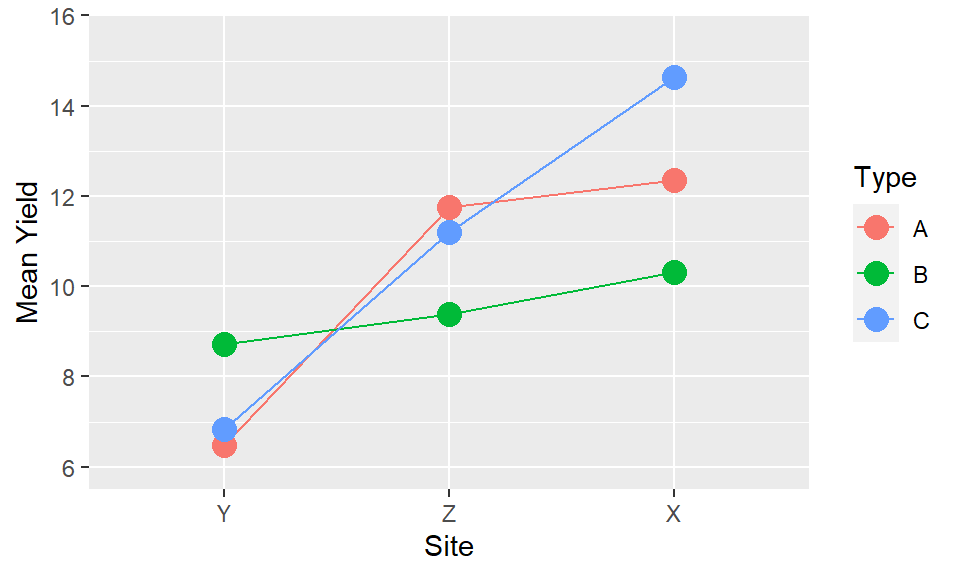
\includegraphics{PresentingResults_files/figure-latex/unnamed-chunk-22-1.pdf}

\hypertarget{step-7-facets}{%
\subsection{Step 7: Facets}\label{step-7-facets}}

\begin{enumerate}
\def\labelenumi{\alph{enumi}.}
\item
  \begin{quote}
  Facets to can make it easier to display even up to four variables simultaneously if we also use a gridded facet layout - e.g.~main interaction of interest showing Type by Inputs; but with row facets corresponding to gender and column facets corresponding to location.
  \end{quote}
\end{enumerate}

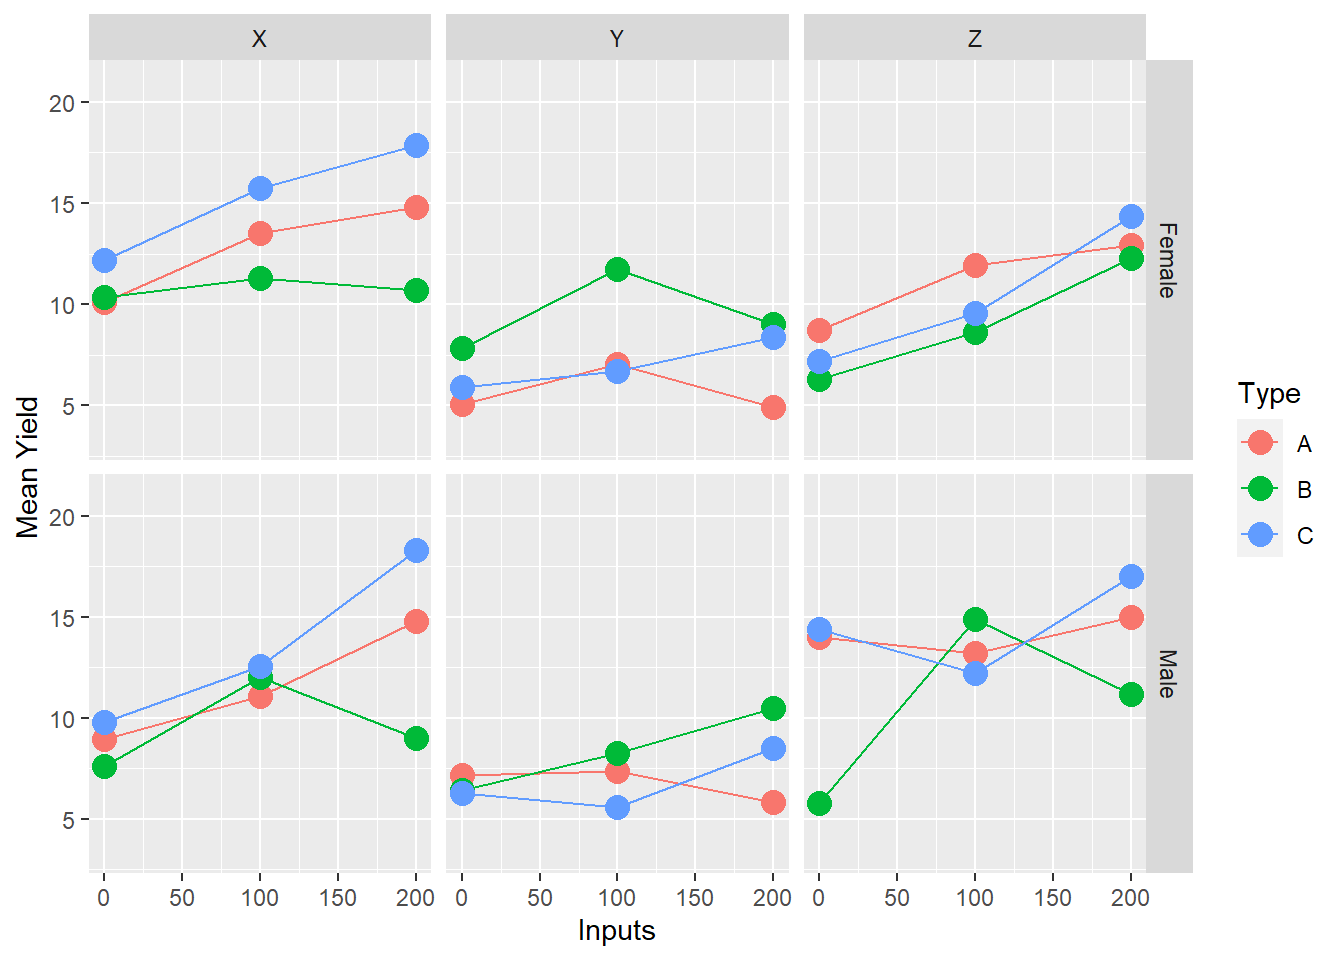
\includegraphics{PresentingResults_files/figure-latex/unnamed-chunk-23-1.pdf}

\hypertarget{step-9-next-steps}{%
\subsection{Step 9: Next steps}\label{step-9-next-steps}}

\begin{enumerate}
\def\labelenumi{\alph{enumi}.}
\item
  \begin{quote}
  Talking to researchers about real experiments almost always leads to discussion about response to one factor (often known) be modified by one or more others. The challenge: find examples where that is not the case!
  \end{quote}
\item
  \begin{quote}
  Statistical significance v practice significance e.g.~a graph of main effects might be useful even if there is statistically significant interaction as long as it is small. But in general if there is a significant interaction we should be looking to display this and not overlook it for the sake of finding an easy answer.
  \end{quote}
\item
  \begin{quote}
  Representing uncertainty. The standard `error bars' on means are actually meaningless for most experimental data. SEDs and CIs of differences better but only easy for neat experiments. See chapter \{LINK\}
  \end{quote}
\item
  \begin{quote}
  Start thinking about labeling, and visual components beyond just the mechanical composition. See chapter \{LINK\}
  \end{quote}
\end{enumerate}

\hypertarget{precision}{%
\chapter{Precision and variability}\label{precision}}

\begin{verbatim}
## Warning in ifelse(fs$adults != "6+", as.numeric(as.character(fs$adults)), : NAs
## introduced by coercion
\end{verbatim}

\hypertarget{section-under-construction}{%
\section{SECTION UNDER CONSTRUCTION}\label{section-under-construction}}

\hypertarget{introduction-2}{%
\section{Introduction}\label{introduction-2}}

When presenting results it can be tempting to focus solely on the main patterns and trends we can identify through our analysis. But we always have to bear in mind the levels of uncertainty we have in those trends, and the underlying variability that will exist around those trends. So it is important to consider how we could incorporate these ideas of precision and variability into the way we present our results to assist our audience by providing as much relevant context to the results as we can.

\hypertarget{video-1}{%
\section{Video}\label{video-1}}

\hypertarget{precision-vs-variability}{%
\section{Precision vs Variability}\label{precision-vs-variability}}

When considering this topic we need to be clear on the difference between \emph{precision} and \emph{variability}. Although these concepts are related, they tell us two different things both of which are important:

Precision refers to the uncertainty in the \emph{estimates} or statistics that we calculate from our data. As the amount of data we have increases the amount of precision we have increases. For example - if we were trying to estimate mean household size based on a sample size of 1, then the precision in that mean would be extremely low. But if we had a sample size of 10,000 households we could estimate the mean from then we would have a much more precise estimate.

Variability refers to the underlying variability in the sample, and in the population. This is not impacted by increasing the sample size, other than that increasing the sample size will increase the precision in our estimates of variability!

\hypertarget{precision-1}{%
\section{Precision}\label{precision-1}}

\hypertarget{confidence-intervals-vs.-standard-errors}{%
\subsection{Confidence intervals vs.~standard errors}\label{confidence-intervals-vs.-standard-errors}}

\hypertarget{in-tables}{%
\subsection{In tables}\label{in-tables}}

\hypertarget{around-trends}{%
\subsection{Around trends}\label{around-trends}}

\hypertarget{overload-of-error-bars}{%
\subsection{Overload of error bars?}\label{overload-of-error-bars}}

\hypertarget{variability}{%
\section{Variability}\label{variability}}

\hypertarget{plots-which-can-display-variability}{%
\subsection{Plots which can display variability}\label{plots-which-can-display-variability}}

\hypertarget{boxplotsviolin-plots}{%
\subsubsection{Boxplots/Violin Plots}\label{boxplotsviolin-plots}}

\hypertarget{histograms}{%
\subsubsection{Histograms}\label{histograms}}

\hypertarget{cumulative-frequency-plots}{%
\subsubsection{Cumulative Frequency Plots}\label{cumulative-frequency-plots}}

\hypertarget{scatter-plots}{%
\subsubsection{Scatter plots}\label{scatter-plots}}

\hypertarget{in-tables.-is-standard-deviation-always-the-answer}{%
\subsection{In tables. Is standard deviation always the answer?}\label{in-tables.-is-standard-deviation-always-the-answer}}

\hypertarget{farmers}{%
\chapter{Presenting results as tables and graphs 4 for farmers}\label{farmers}}

\hypertarget{section-under-construction-1}{%
\section{SECTION UNDER CONSTRUCTION}\label{section-under-construction-1}}

\hypertarget{papers}{%
\chapter{Presenting in papers}\label{papers}}

\hypertarget{section-under-construction-2}{%
\section{SECTION UNDER CONSTRUCTION}\label{section-under-construction-2}}

\hypertarget{posters}{%
\chapter{Presenting on posters}\label{posters}}

\emph{Alex Thomson}

\hypertarget{video-2}{%
\section{Video}\label{video-2}}

\hypertarget{the-aim-of-posters}{%
\section{The aim of posters}\label{the-aim-of-posters}}

Academic research posters are a great way to engage with your scientific community by succinctly distilling your research onto a large display, crowded by your peers doing just the same.

These could be shown off in many different settings.

\begin{itemize}
\tightlist
\item
  Large scientific (inter-disciplinary) conferences
\item
  Smaller conferences devoted mostly to your field
\item
  Social media channels such as Twitter
\item
  Small online meetings with fixed presentation schedules
\item
  Blogs
\item
  Other online settings such as Miro
\end{itemize}

Regardless of the setting, the sharing of research posters is designed to be a learning experience for both the presenter and the audience.

\textbf{\emph{For the presenter}},

\begin{itemize}
\tightlist
\item
  Share their research with the wider academic community
\item
  Engage directly with their colleagues
\item
  Receive feedback from their peers
\item
  Develop their presentation and communication skills
\item
  Networking opportunities
\end{itemize}

\textbf{\emph{For the audience}},

\begin{itemize}
\tightlist
\item
  Learn about the research currently happening within their community
\item
  Engage directly with their colleagues
\item
  Potentially gain insights which could aid in their own research
\item
  Networking opportunities
\end{itemize}

\hypertarget{key-principles}{%
\section{Key principles}\label{key-principles}}

\hypertarget{the-importance-of-design-and-layout}{%
\subsection{The importance of design and layout}\label{the-importance-of-design-and-layout}}

Crucial to ensuring the effectiveness of your poster and making sure you are calable of attracting an audience for your poster.

For a virtual conference, you may not have to fight for an audience but you still will need to keep their attention and keep them interested.

An inaccessible or poor design can be very off putting.

\begin{itemize}
\tightlist
\item
  Put your sections into a logical flow so the audience knows where to read
\item
  Avoid the dreaded ``Wall of text''
\item
  Avoid clutter, keep it tidy
\item
  Avoid using images as a background
\item
  Keep your colours and text consistent
\end{itemize}

Always think carefully about what might be expected by your audience and what might keep them entertained.

If possible, always reach out for feedback on a draft before creating a final poster.Friends, family, colleagues, supervisors, anyone.

There are a couple base design types that have become common over the years.

\textbf{\emph{Traditional Design}}

\begin{center}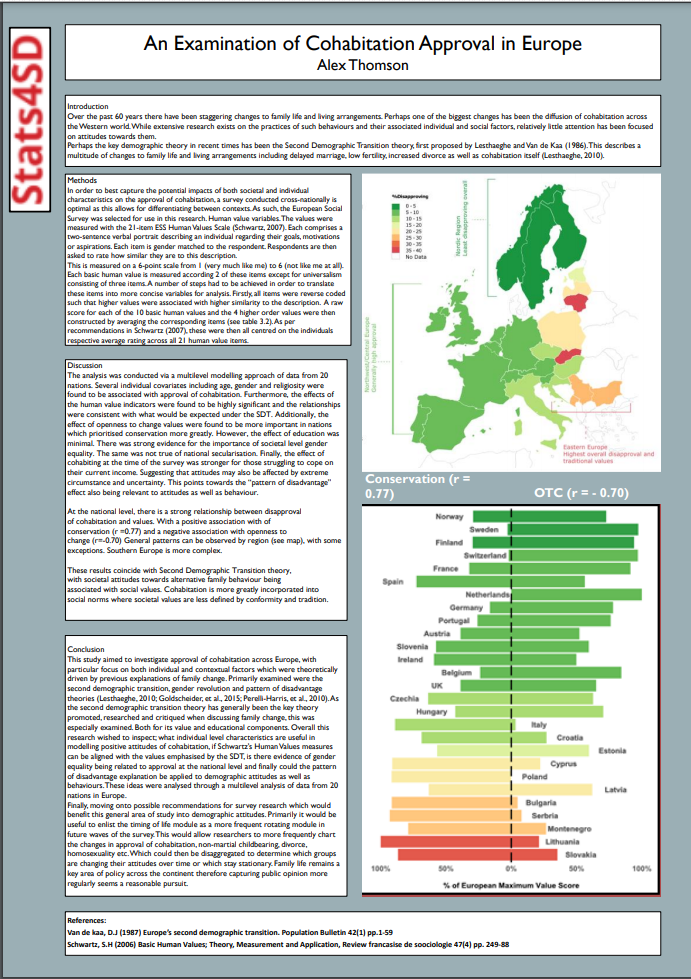
\includegraphics[width=9.6in]{img/trad example 1} \end{center}

Traditional Poster Example Auothr: Alex Thomson (Note: Crude example of design, not all text is relevant)

Each section within individual text boxes arranged into 2/3 columns oriented portrait or landscape.

This traditional design dominates most poster conferences and will likely be the most common format for any template posters you find online.

\textbf{Strengths}

\begin{itemize}
\tightlist
\item
  Useful for audiences requiring lots of detail
\item
  Requires little application of creative/graphic design
\item
  Easy to read and follow the order
\item
  The basis for most templates
\end{itemize}

\textbf{Weaknesses}

\begin{itemize}
\tightlist
\item
  Can appear lazy simply because of how common this format is
\item
  Often encourages the ``Wall of text''
\item
  Requires creativity in order to make this stand out
\item
  Gaining attention relies more heavily on the title and imagery
\item
  Common for people to just copy and paste from report into a template when using this design
\end{itemize}

\begin{figure}
\centering
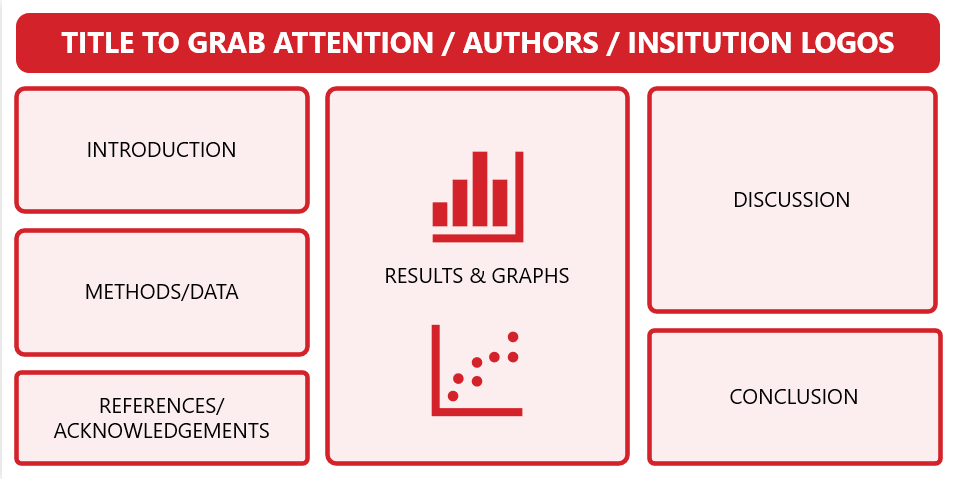
\includegraphics{img/Traditional Poster design template.png}
\caption{Traditional Poster Design template}
\end{figure}

\textbf{\emph{\#betterposter design}}

Suggested by American PhD student Mike Morrison in a series of videos critical of the traditional approach and design to posters.

This has become a larger campaign being take up in real world applications and with plans in the works to conduct full studies into its efficacy.

The approach takes a user experience approach to poster design to increase the size of a potential audience, improve readability and more memorable.

This is done by putting overwhelming emphasis on the key findings and results with these taking up the majority of the space on the page.

This is put in the center in plain language, supplemented by imagery, with information bars either side.

The left panel (\emph{silent presenter}) bullet points much of the normal information you would expect to find.

While the right panel (\emph{ammo bar}) is filed with additional information that find the study particularly interesting and largely used when the presenter is answering questions.

\begin{figure}
\centering
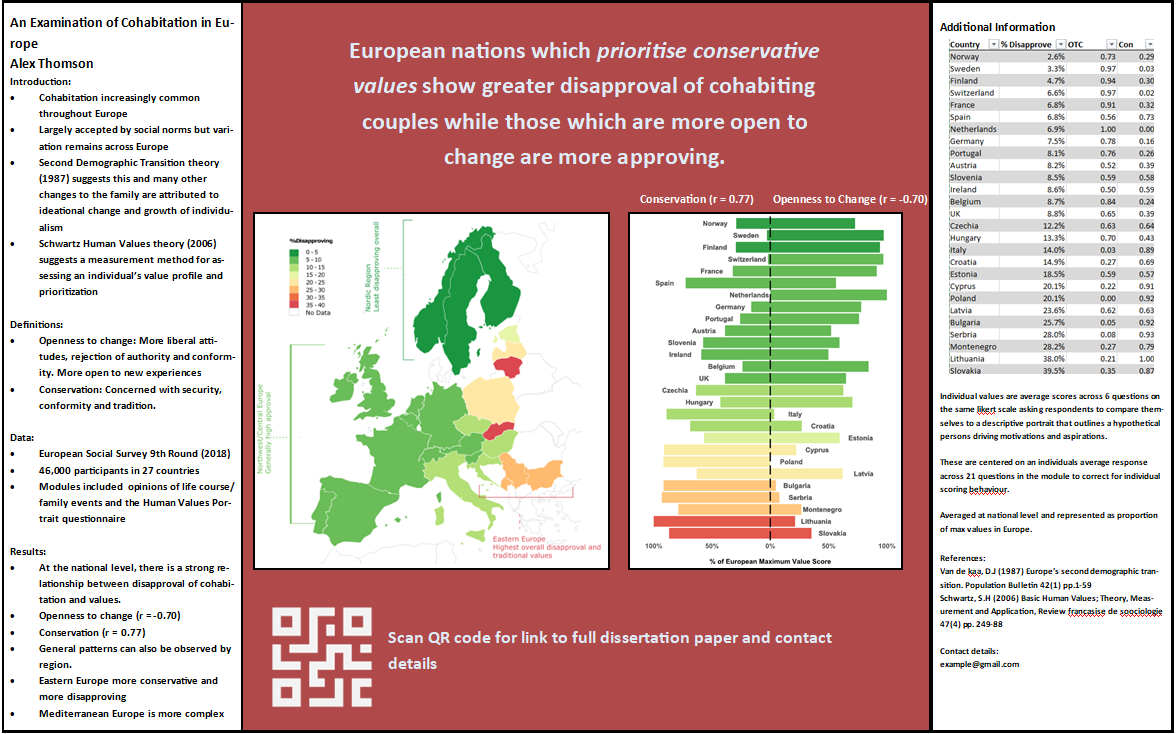
\includegraphics{img/better poster example 1.png}
\caption{\#betterposter Example Author: Alex Thomson}
\end{figure}

\textbf{Strengths}

\begin{itemize}
\tightlist
\item
  Avoids overloading the reader with information.
\item
  Strongly limits the word count.
\item
  Simple design to work with.
\item
  QR codes can be included to link to copies of the poster, the study and contact details.
\item
  Attracts the audience in with a key interesting statement.
\item
  Tends to be written in more plain language than other posters, ignoring scientific jargon.
\item
  More approachable to a wider variety of people.
\item
  Less information means more likely to be remembered by the audience.
\end{itemize}

\textbf{Weaknesses}

\begin{itemize}
\tightlist
\item
  Mostly designed for in-person conferences.
\item
  QR code being included assumes there are additional resources to link to. Not always the case.
\item
  To a more critical audience, may appear simple and reductive.
\item
  Still a new approach so may be a off-putting to some stuck in traditional ways
\item
  Assumes you have a key finding to present.
\item
  May not be as appropriate for posters not designed for studies or those which prioritise methods
\item
  ``Ammo bar'' assumes presence of a knowledgeable presenter
\end{itemize}

Although you do not have to follow its format exactly if you do not feel comfortable using it. The principles behind its creation are sound and should be considered regardless of your design. Using a user design experience approach, the campaign suggests;

\begin{itemize}
\tightlist
\item
  Limiting the amount of information presented. Focus on the most important information.
\item
  Making the poster easier and quicker to read
\item
  Making the experience more useful to the audience, less information means they can make the most out of their time and look at more posters
\item
  Removing any barriers to your poster. Things that will stop someone from wanting to read it.
\end{itemize}

There will be other ways to achieve these same goals.

\begin{figure}
\centering
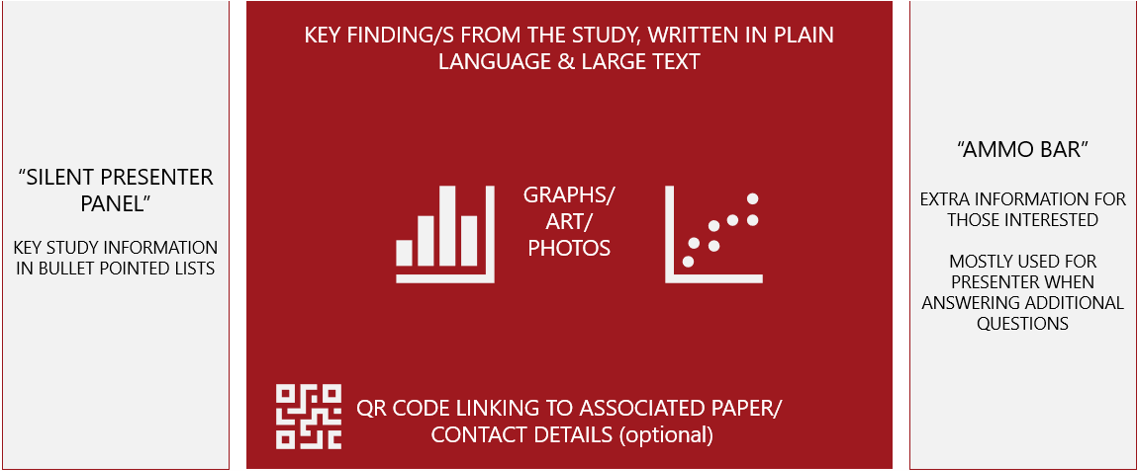
\includegraphics{img/Better Poster template.png}
\caption{\#betterposter template}
\end{figure}

\textbf{\emph{Infographics}}

Infographics are posters designed to provide lots of information and facts to the audience. Or alternatively to visually display some kind of theory/principle in an interesting way.

Usually requires high levels of creative design over graphics and images. Usually with the help of a graphic designer.

Can help in generating discussion of a complex subject.

Could be useful in providing context of an upcoming study, generating an argument for the importance of an upcoming study or reporting the initial descriptive results from a large survey.

Assumes generally you have lots and lots of interesting numbers, results and facts to tell the audience. Or a theory which is easy to show off visually.

Can be off-putting to supply the audience with so much information at once.

\begin{center}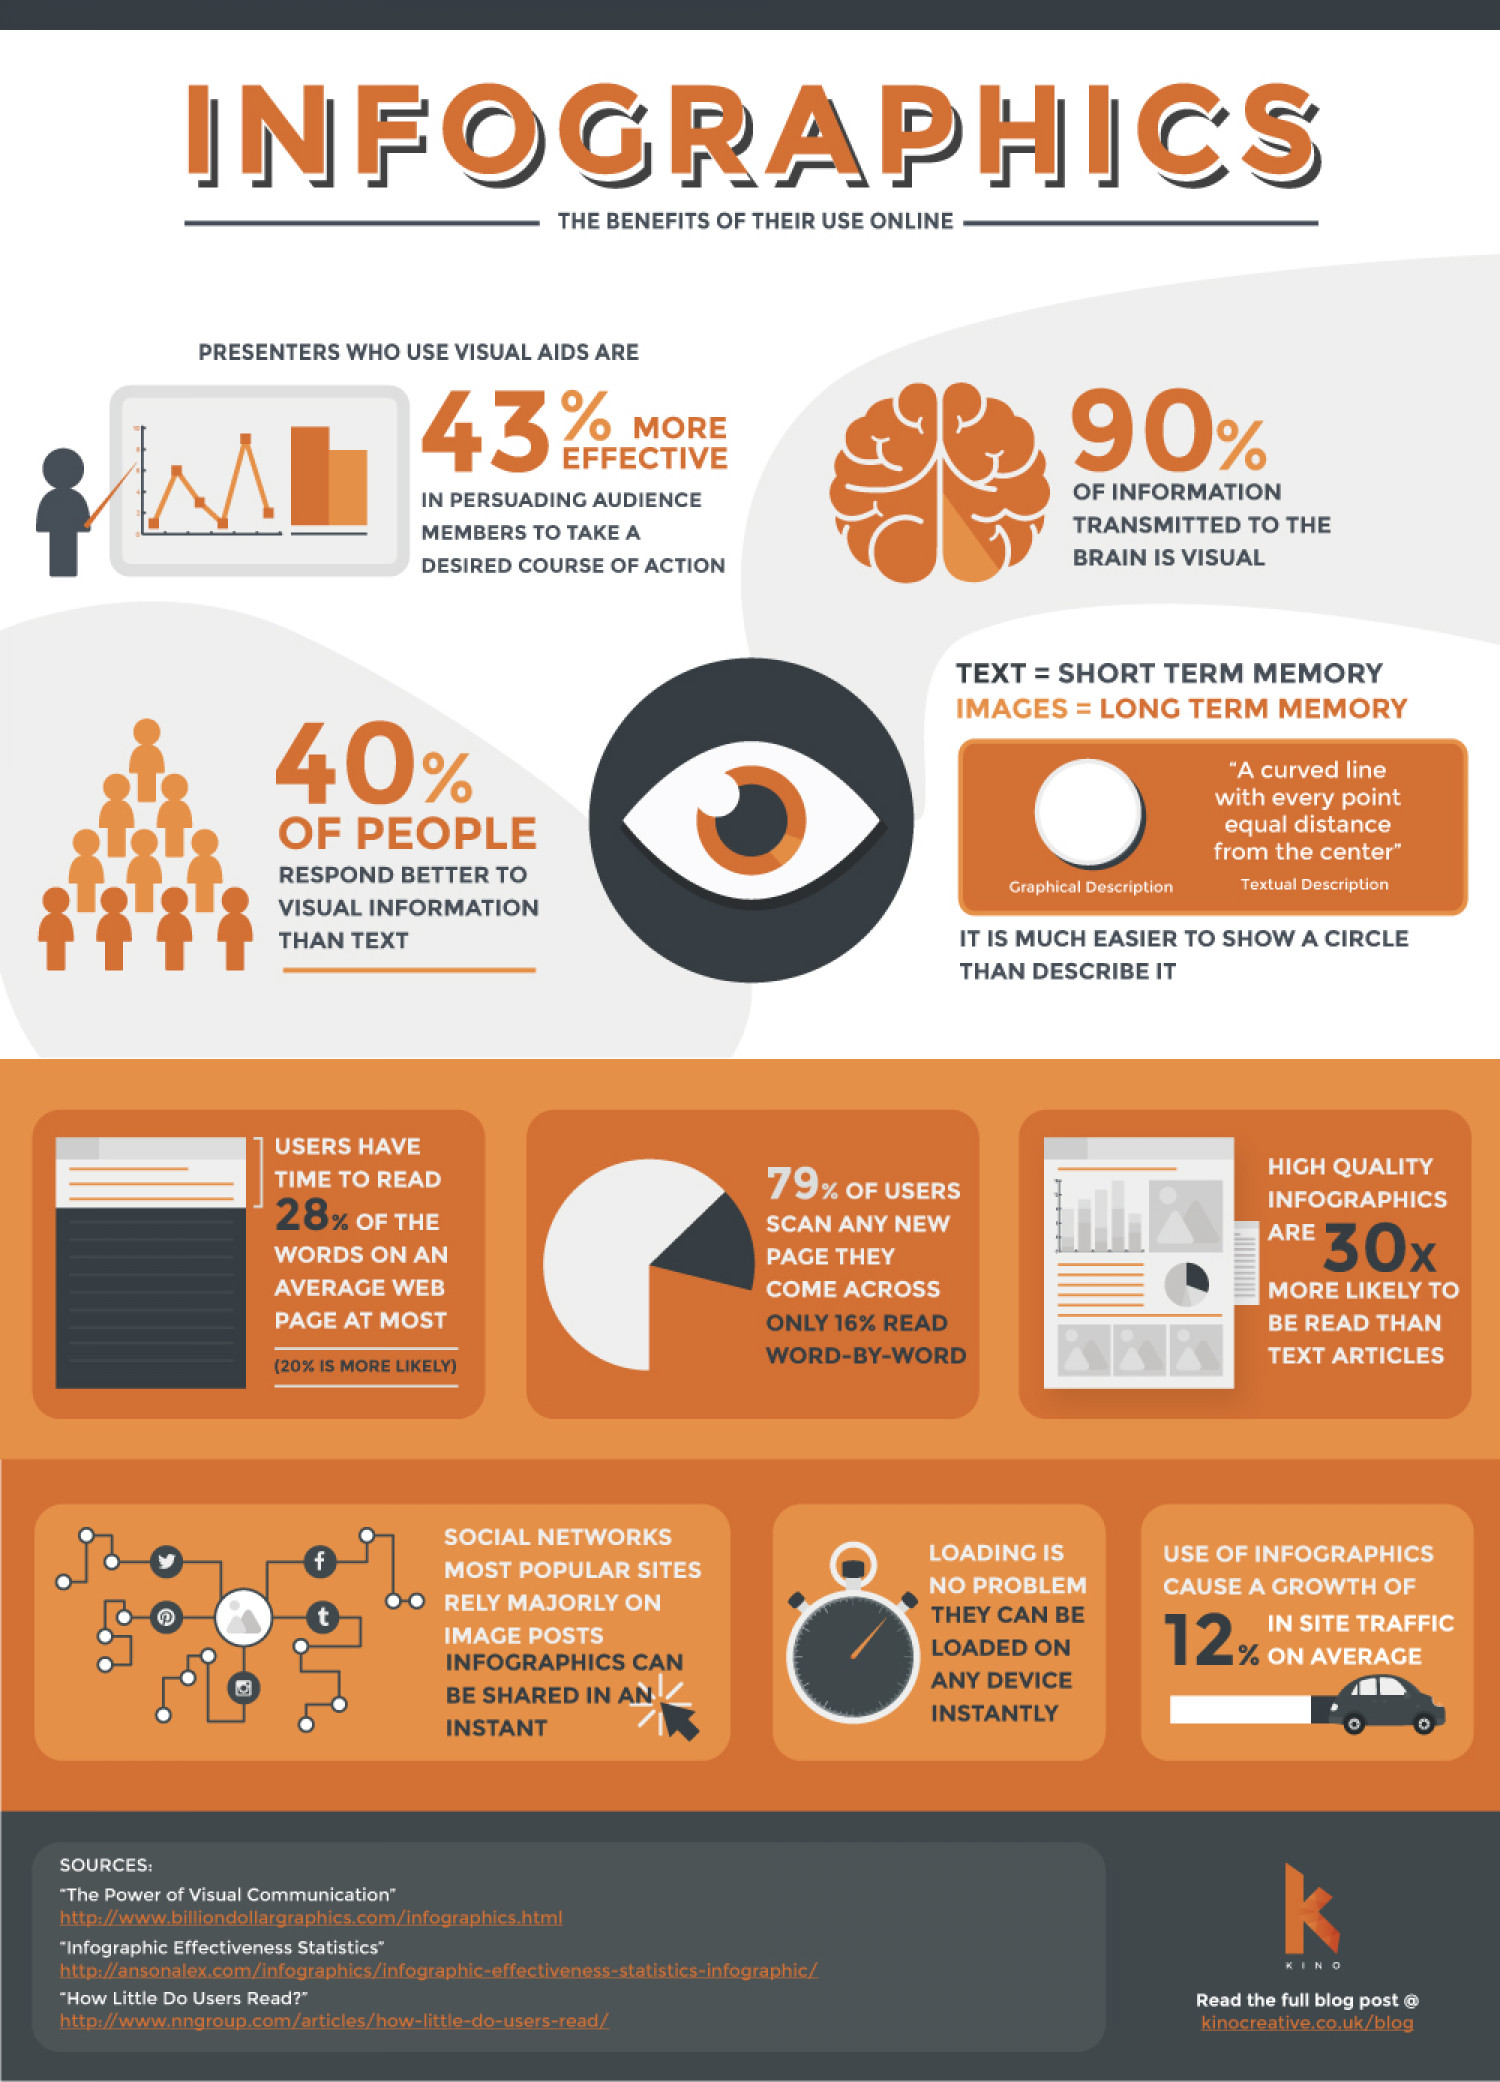
\includegraphics[width=0.5\linewidth,height=0.25\textheight]{img/infographic} \end{center}

\href{https://visual.ly/community/Infographics/technology/infographics-benefits-their-use-online?utm_source=visually_embed}{Source of infographic: Visual.ly}

\textbf{\emph{Be creative}}

Your options are not limited to these ideas. Always be thinking about how you could \textbf{\emph{be creative}}

Your choices can be expanded or constrained by the setting and rules of your poster session.

\emph{Consider the follwing questions and ideas}

\begin{itemize}
\tightlist
\item
  Are you allowed interactive elements?

  \begin{itemize}
  \tightlist
  \item
    Screens? Could include video
  \item
    Handouts?
  \item
    Physical models?
  \end{itemize}
\item
  Are they displayed on screens or paper?

  \begin{itemize}
  \tightlist
  \item
    on screens could be turned into an animated presentation
  \end{itemize}
\item
  Is it a virtual conference?

  \begin{itemize}
  \tightlist
  \item
    Do you have a scheduled presentation slot?
  \item
    If so, engagement more reliant on your presentation skills and content over design
  \item
    Is it on twitter?
  \item
    Think about how you can use the medium to your advantage
  \item
    Promote yourself and your poster
  \item
    Could animate your poster as a GIF
  \item
    Use the text to include additional contextual information not on the poster
  \end{itemize}
\end{itemize}

\hypertarget{keep-it-short-and-simple}{%
\subsection{Keep it short and simple}\label{keep-it-short-and-simple}}

Avoid the temptation to summarise every little thing about your study. You should be thinking about your poster as a \textbf{visual abstract}. Something to advertise your research and your skills.

\begin{itemize}
\tightlist
\item
  Focus on just \textbf{one or two key messages} about your study

  \begin{itemize}
  \tightlist
  \item
    This could be key findings or interesting innovations/applications of your methodology
  \end{itemize}
\item
  Prioritise including information that the audience \textbf{needs} to know first
\item
  Only include information on the poster that is relevant to these key messages

  \begin{itemize}
  \tightlist
  \item
    You may have the chance to highlight other parts of your study when asked questions by audience members
  \end{itemize}
\end{itemize}

\begin{quote}
``It seems that perfection is attained not when there is nothing more to add, but when there is nothing more to remove'' Antoine de Saint Exupery \footnote{Quoted originally in the \#betterposter videos}
\end{quote}

Use this quote as a guiding rule. Always ask yourself what is \emph{needed}, \emph{relevant}, and \emph{engaging}.

There is no set rule when it comes to a word count although the rules of your session/conference may dictate one which you should follow.

\begin{itemize}
\tightlist
\item
  Some resources will say keep it under 1,000 words \footnote{Colin Purrington blog, see link above}
\item
  Others around 300 - 800 \footnote{NYU guide, see link above}
\item
  One guide even suggests restricting yourself down to just 250 \footnote{LSE guide, see link above}
\end{itemize}

The best advice that can be given here is to consider how much you are comfortable saying and how much it is you have to say, as well as think about what might the audience be expecting.

The following sections are the standard parts to include for a research poster although what you need to include may depend on your purpose and how far along in your study you are.

\textbf{\emph{Introduction}}

\begin{itemize}
\tightlist
\item
  Make this something quick to \textbf{grab the readers attention}
\item
  Let them know \emph{why} they should keep reading
\item
  Get across the point and relevance of your study
\item
  Perhaps draw them in with a hypothesis/research question
\end{itemize}

\textbf{\emph{Methods/Approach}}

\begin{itemize}
\tightlist
\item
  To some this may actually be the most interesting part, especially if your method is quite innovative

  \begin{itemize}
  \tightlist
  \item
    if so, be sure to give this section great attention so you can explain why your method is special
  \end{itemize}
\item
  Otherwise, keep this section brief to focus on your findings and interpretations
\item
  Where possible, display your approach through a diagram or pictures.

  \begin{itemize}
  \tightlist
  \item
    Especially if the study was an experimental design or a trial
  \end{itemize}
\end{itemize}

\textbf{\emph{Results}}

\begin{itemize}
\tightlist
\item
  This will likely take up more space on the poster than any other section
\item
  Only include the most interesting and relevant findings

  \begin{itemize}
  \tightlist
  \item
    Don't include anything that doesn't \textbf{need} to be there
  \end{itemize}
\item
  Unless your study was using qualitative data analysis, this section will likely include only short sentences
\item
  Use graphs, maps, and tables which help to illustrate the key findings and messages
\end{itemize}

\textbf{\emph{Discussion/Conclusion}}

\begin{itemize}
\tightlist
\item
  Some will choose to separate these two into different sections
\item
  Focus only on interpreting your most relevant and interesting results
\item
  Try to explain what your findings mean in plain language.
\item
  The audience will want to know \emph{why} your results are important and interesting
\end{itemize}

\textbf{\emph{References}}

\begin{itemize}
\tightlist
\item
  Always to be included if you reference any material on your poster
\item
  Keep this small and to the bottom of the page
\end{itemize}

\textbf{\emph{Acknowledgements}}

\begin{itemize}
\tightlist
\item
  Acknowledge your institution, employer, tutors and any colleagues who aided you.
\item
  Good to provide contact details to keep up engagement after the session
\end{itemize}

\hypertarget{make-it-engaging}{%
\subsection{Make it engaging}\label{make-it-engaging}}

If your poster is displayed at a conference, in person or online, you may be fighting for attention with hundreds of other posters within a limited time frame.

You must attract and engaging.

Think about your poster as an advert for your research. What can you include to draw in potential ``customers''?, how can you make them remember you?

This will come down to both your presentation and design of your poster as well as the interactions you have with your audience.

\textbf{\emph{Tips to engage with your presentation}}

\begin{itemize}
\tightlist
\item
  Grab them with your title. Consider making the title a statement of your key finding
\item
  Use imagery

  \begin{itemize}
  \tightlist
  \item
    Photos
  \item
    Graphs
  \item
    Diagrams
  \item
    Maps
  \end{itemize}
\item
  Don't use too many graphs
\item
  Don't use overly-complicated hard to read graphs
\item
  Avoid tables where possible

  \begin{itemize}
  \tightlist
  \item
    Keep them simple if they are used
  \end{itemize}
\item
  Avoid complicated inaccessible language

  \begin{itemize}
  \tightlist
  \item
    Broad plain language will be understood by a larger audience
  \end{itemize}
\item
  Use colour effectively

  \begin{itemize}
  \tightlist
  \item
    Don't use too many different colours. Pick a couple to design a colour palette/scheme
  \item
    Avoid overly saturated colours
  \end{itemize}
\item
  Be creative with your medium

  \begin{itemize}
  \tightlist
  \item
    Can you use interactive screens?
  \item
    Using twitter? Could animate your presentation as a GIF
  \end{itemize}
\end{itemize}

Also think about the information that you include on your poster.

\textbf{\emph{What information is going to trigger interesting conversations with your audience?}}

\begin{itemize}
\tightlist
\item
  Hypotheses
\item
  Research Questions
\item
  Surprising results
\item
  Important recommendations
\item
  New theories/models?
\item
  Ask the audience questions to make them think
\end{itemize}

\textbf{\emph{Tips to engage with your interactions}}

\begin{itemize}
\tightlist
\item
  Be prepared in advance to answer any and all questions
\item
  Include your contact details prominently on your poster
\item
  Consider printing out smaller hand out versions of your poster
\item
  Details on where to find the paper and poster online
\item
  Keep notes with additional notes at hand that you can refer to
\item
  Advertise your poster beforehand using social media
\end{itemize}

\hypertarget{some-examples}{%
\subsection{Some examples}\label{some-examples}}

\begin{figure}
\centering
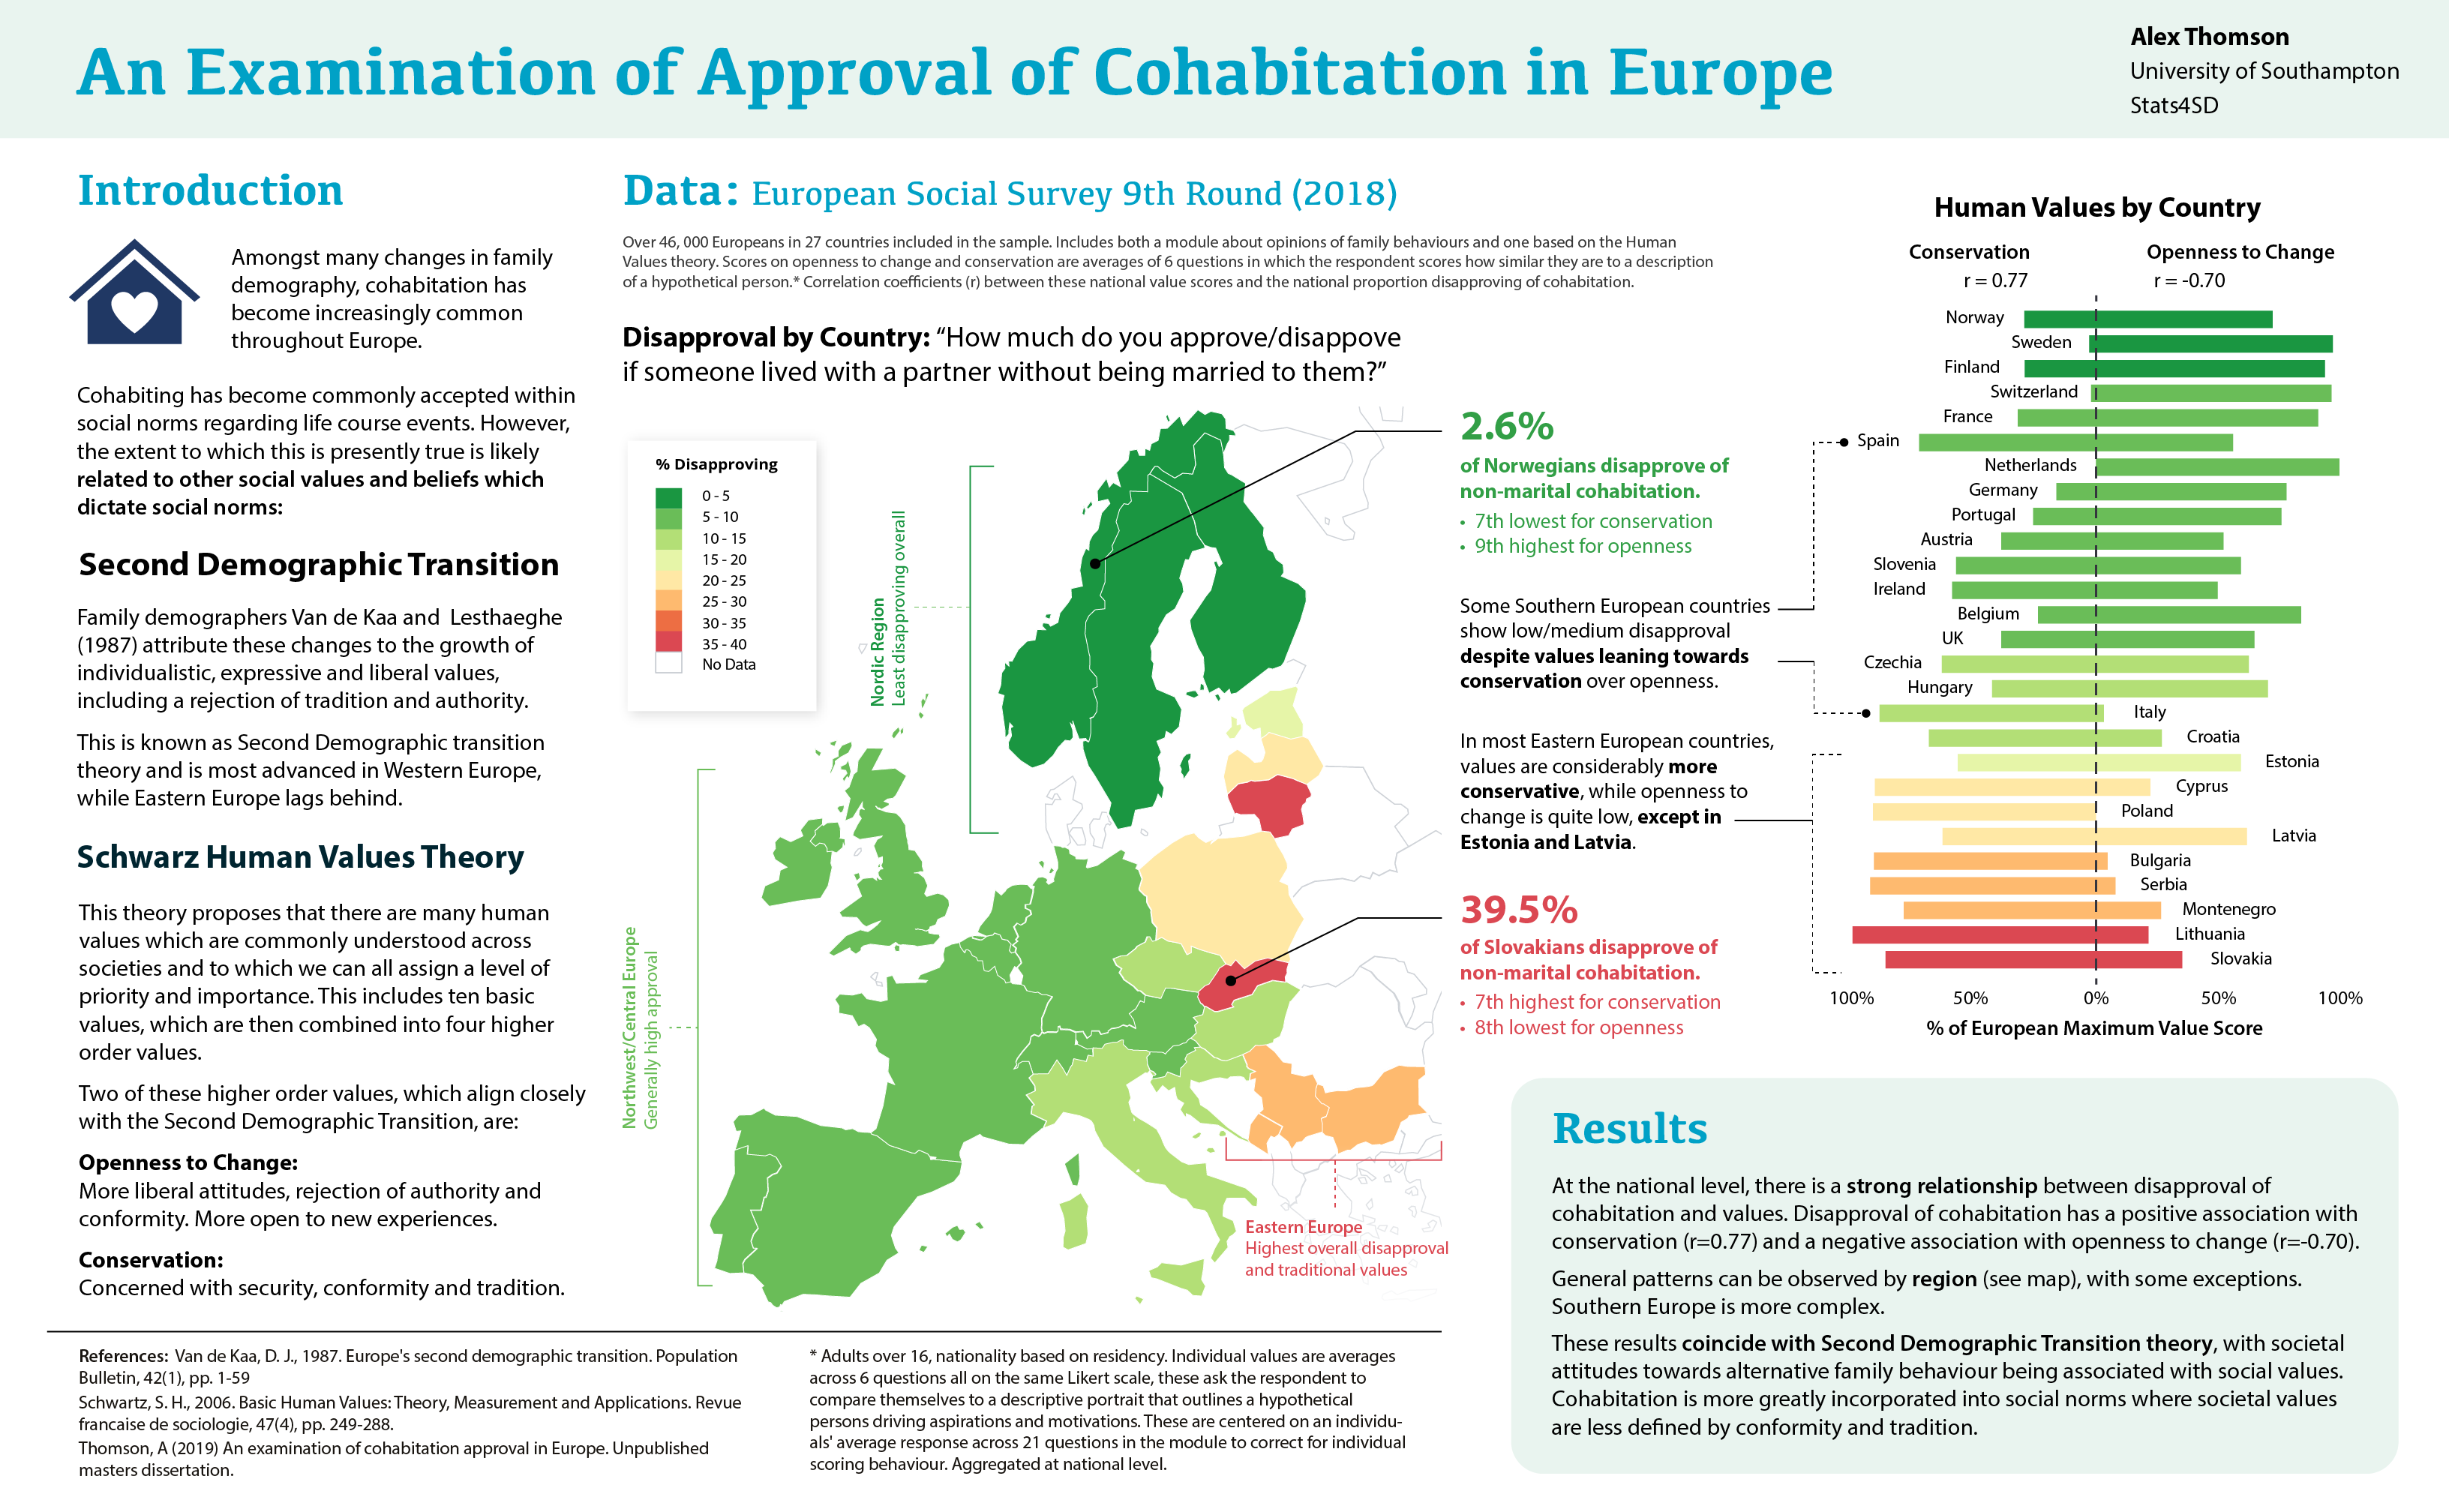
\includegraphics{img/YISA Poster 2020.png}
\caption{Example 1: Our compeition winning twitter poster Authors: Alex Thomson and Emily Nevitt}
\end{figure}

This poster keeps the word count short to less than 300 words, down from a dissertation over 19,000 words, and picks out just two key descriptive findings

Maps and an interesting graph dominate the page to draw in the audience.

\begin{figure}
\centering
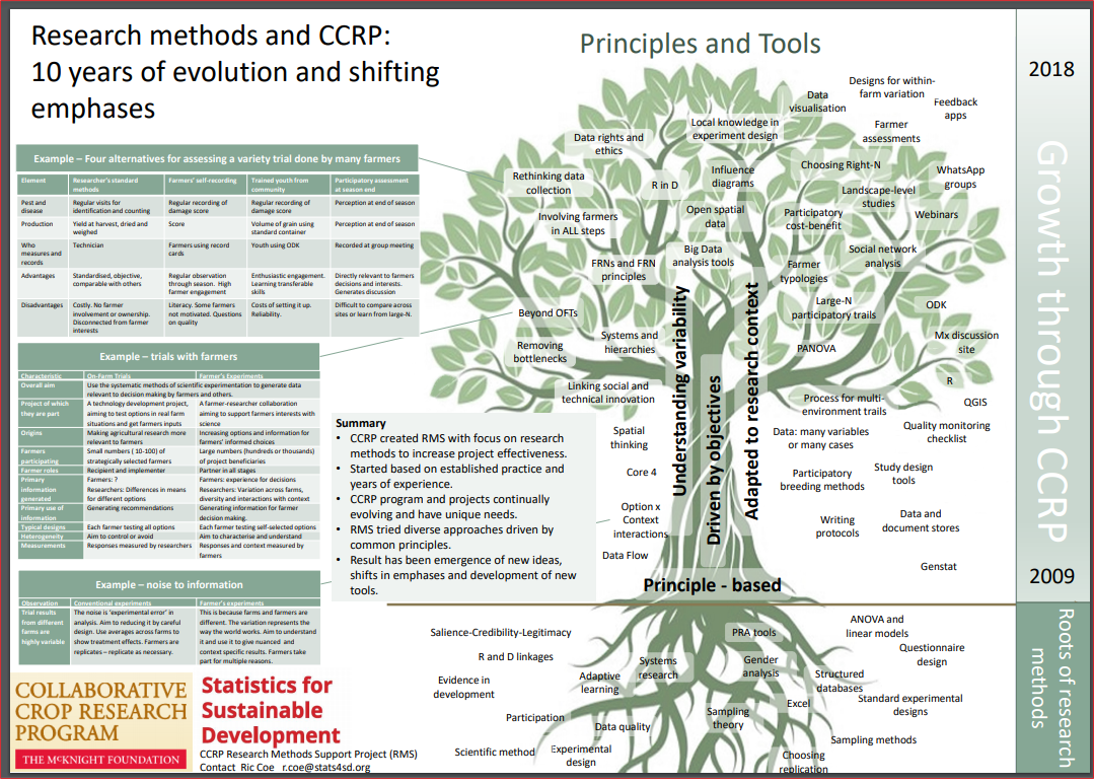
\includegraphics{img/CCRP poster 1.png}
\caption{Example 2: RMS Poster Author: Ric Coe}
\end{figure}

A large interesting diagram draws the eye

Shows that research and studies is not the only reason to make a poster as this is designed to illustrate key principles, examples and practices.

\begin{center}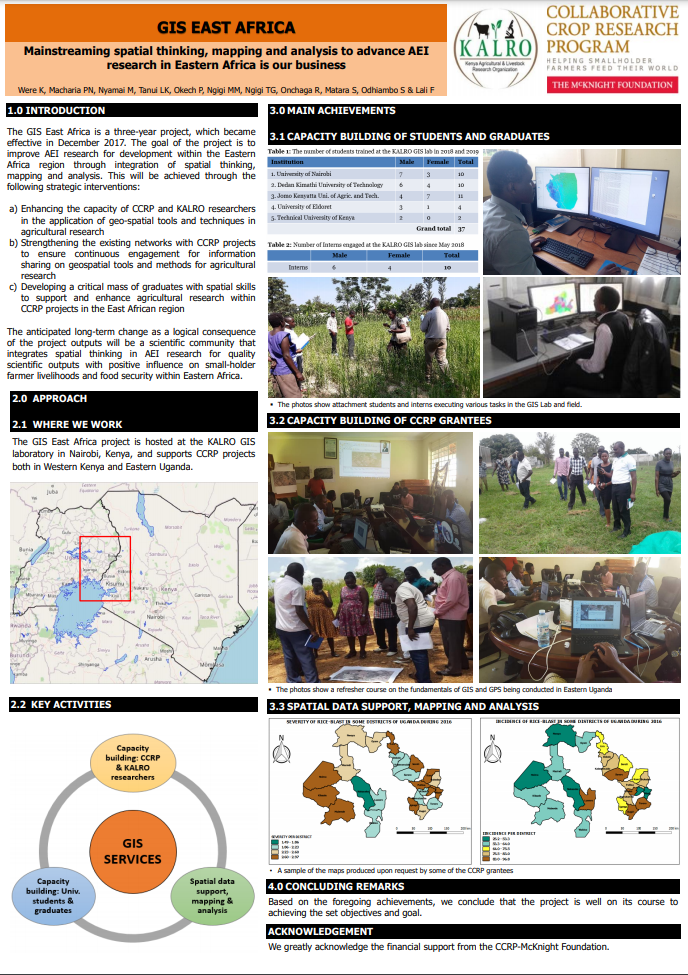
\includegraphics[width=9.56in]{img/GIS East Africa Poster} \end{center}

Example 3: CCRP Poster - GIS East Africa Authors: Were K, Macharia PN, Nyamai M, Tanui LK, Okech P, Ngigi MM, Ngigi TG, Onchaga R, Matara S, Odhiambo S and Lali F

Again it is kept short and simple with many photos, maps and diagrams used to succinctly illustrate the key messages.

\begin{figure}
\centering
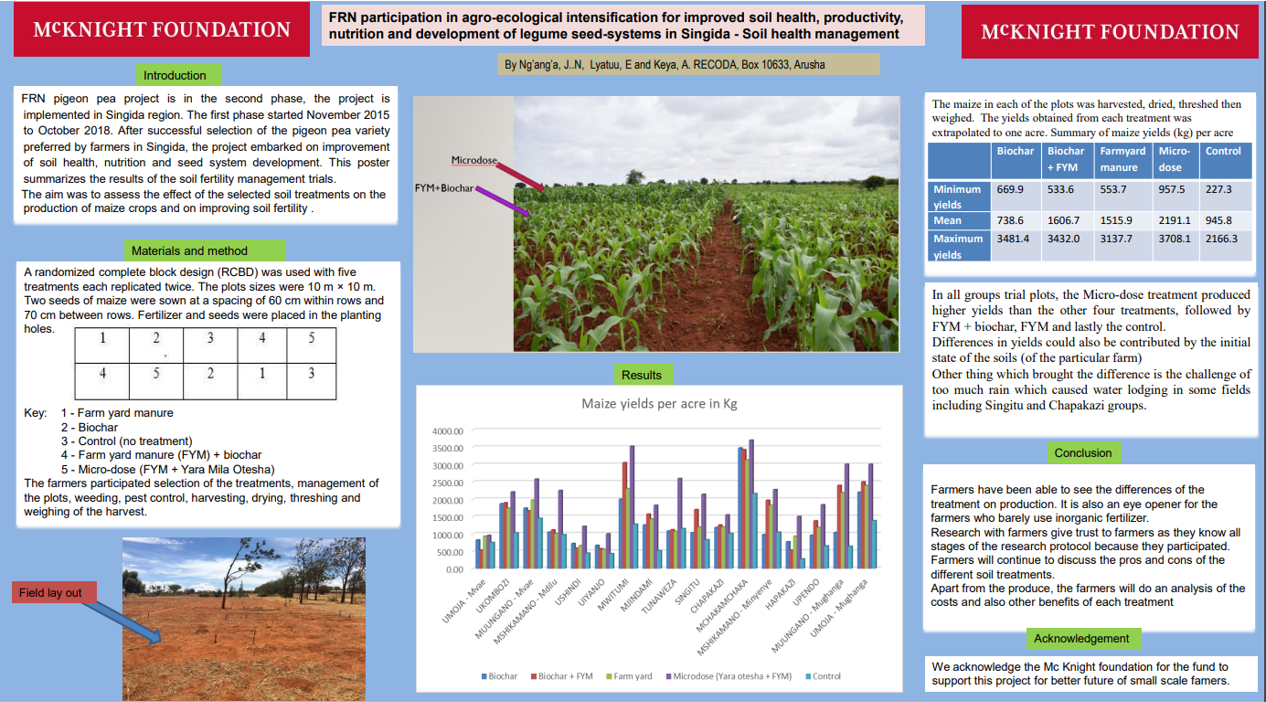
\includegraphics{img/Pigeon Pea FRN.png}
\caption{Example 4: CCRP Poster - Pigeon Pea FRN Authors: Ng'ang'a J, Layatuu E and Keya A}
\end{figure}

A smart use of the traditional design keeping the word count fairly low and choosing plenty of imagery to illustrate the results and methodology.

\begin{figure}
\centering

\includegraphics{img/Sorghum Kenya.png}
\caption{Example 5: CCRP Poster - Sorghum Kenya Authors: F. Wamunga, A. Were, E.J Too, B.O Nyongesa, F.Odiwuor, E. Ouma, S. Gudu}
\end{figure}

Makes use of the traditional design also with good use of imagery and space, very informative and includes all relevant sections. Arguably may include too much text however.

\hypertarget{other-resources-1}{%
\subsection{Other resources}\label{other-resources-1}}

\emph{Colin Purrington Blog filled with plenty of tips, dos and dont's and templates}

\href{https://colinpurrington.com/tips/poster-design/}{Blog}

\href{https://colinpurrington.com/2019/06/templates-for-better-posters/}{Templates}

\emph{Some helpful guides provided by universities}

\href{https://guides.nyu.edu/posters}{New York University}

\href{https://www.reading.ac.uk/web/files/dps/Conference_poster_PPT_examples.pdf}{University of Reading}

\href{https://blogs.lse.ac.uk/impactofsocialsciences/2018/05/11/how-to-design-an-award-winning-conference-poster/}{London School of Economics}

\href{http://www.supi.manchester.ac.uk/forteachers/academicposterguidance/}{University of Manchester}

\href{https://urc.ucdavis.edu/creating-effective-academic-posters}{UC Davis}

\emph{\#betterposter campaign}

\href{https://www.youtube.com/watch?v=1RwJbhkCA58\&t=2s\&ab_channel=MikeMorrison}{Video 1}

\href{https://www.youtube.com/watch?v=SYk29tnxASs\&ab_channel=MikeMorrison}{Video 2}

\href{https://www.youtube.com/watch?v=fQDL8r3r_d4\&ab_channel=MikeMorrison}{Video 3: Twitter Posters}

\href{https://www.insidehighered.com/news/2019/06/24/theres-movement-better-scientific-posters-are-they-really-better}{Response Article}

\emph{Whole website devoted to academic research posters}

\href{https://www.academicposter.org/}{Acedemicposter.org}

\href{https://www.posterpresentations.com/index.html}{PosterPresentations.com}

\emph{Academic Papers}

\href{https://febs.onlinelibrary.wiley.com/doi/epdf/10.1111/febs.13383}{Rowe and llic: Rethinking poster presentations at large-scale scientificmeetings -- is it time for the format to evolve?}

\href{https://www.sciencedirect.com/science/article/pii/S2049080116301303}{Gundogan et al: How to make and academic poster}

\href{https://www.ncbi.nlm.nih.gov/pmc/articles/PMC1955747/}{Miller Preparing and Presenting Effective Research Posters}

\textbf{\emph{Examples}}

\emph{Pintrest boards}

\href{https://www.pinterest.co.uk/jing4717/academic-poster/}{Board 1}

\href{https://www.pinterest.at/tzesire/conference-posters-design/}{Board 2}

\emph{Other}

\href{https://ur.umbc.edu/poster-presentation-examples/}{UMBC collection of inter-disciplinary examples}

\emph{Template collections}

\href{https://templatelab.com/research-posters/}{Template Lab}

\hypertarget{audience1}{%
\chapter{Adapting to the audience}\label{audience1}}

\hypertarget{draft-2}{%
\section{DRAFT}\label{draft-2}}

\hypertarget{video-3}{%
\section{Video}\label{video-3}}

\hypertarget{without-a-conscious-effort-a-presentation-is-unlikely-to-be-well-adapted-to-its-audience}{%
\section{Without a conscious effort, a presentation is unlikely to be well adapted to its audience}\label{without-a-conscious-effort-a-presentation-is-unlikely-to-be-well-adapted-to-its-audience}}

When we prepare a presentation, it is easy to simply imagine ourselves as the audience and use this perspective to decide what to show and how. Unfortunately, we are not at all a good representative sample of our future audience because:

\begin{itemize}
\tightlist
\item
  We already know what the presentation is about
\item
  Even if we imagine knowing nothing about the content of the presentation, we can't help but imagine someone with a knowledge, background and way of reasoning that is similar to ours\ldots{} and that kind of person cannot be representative of the audience either.
\end{itemize}

So, when we prepare a presentation, it is very important that we make a conscious effort of adapting it to our audience. Otherwise, we're likely to lose it at some point or another. Here are the reasons why:

\begin{enumerate}
\def\labelenumi{\arabic{enumi}.}
\item
  \textbf{Your audience comes with a specific background} Some might be researchers, other might be students. They might be working in the same field, but maybe in a different context, or they might also be working on a completely different field. And we need to adapt the presentation to the diversity of the backgrounds. That's probably the most obvious of the things to be aware of when presenting results.
\item
  \textbf{The audience know less than we think they know} What I mean by that is not that they know very little. They might actually know a lot about the topic, maybe even more than you, but their knowledge will always come from a perspective and experience that is different from yours. And in the end, they will nearly always be weaker than you think in terms of knowledge that align with your personal approach to things. So when you try and evaluate the knowledge level of your audience, keep in mind that your evaluation is always too optimistic.
\item
  \textbf{The audience is not in our brain} - we can't assume that a reasoning process that makes sense to us will automatically make sense to them. So, we always need to guide the audience in our reasoning process, even when it seems obvious to us.
\item
  \textbf{We are not in the audience's brain either} - naturally they will not look exactly where we want them to look at and they will likely be distracted by things that would not necessarily distract us. And so here again, we need to account for it and guide them, so that they stay with us at all time throughout the presentation.
\end{enumerate}

\hypertarget{so-what-to-do}{%
\section{So what to do?}\label{so-what-to-do}}

Here are some things you can do to address each the points raised above:

\hypertarget{our-audience-comes-with-a-specific-background-different-from-ours}{%
\subsection{1. Our audience comes with a specific background, different from ours}\label{our-audience-comes-with-a-specific-background-different-from-ours}}

To address the issue of the audience coming with a specific background,
- Try to use terms and vocabulary that will be understood by everyone - avoid jargon and acronyms.
- Try to put yourself in the shoes of each type of person likely to be there as your audience. And simply ask yourself ``If I had this particular background, What would help me to follow the presentation?''
- Be sure to clearly explain all the things without which someone would not be able to follow the presentation. Buuuut I remind you - don't forget about time and so really focus on explaining \textbf{only} the things that are absolutely necessary to follow the presentation. Be very selective about what you say, and when in doubt, skip it.
That is -\textgreater{} Say little, but say it very clearly! (and keep the rest for the questions)

\hypertarget{our-audience-know-less-than-we-think-they-know}{%
\subsection{2. Our audience know less than we think they know}\label{our-audience-know-less-than-we-think-they-know}}

\begin{itemize}
\tightlist
\item
  Double-check the key parts of your script. These things that are necessary to follow your presentation. Will someone who has only very basic knowledge about the area be able to follow it?
  o If you're not totally sure whether something essential in your presentation is clear enough, then it's probably not clear enough. Make it clearer. If your presentation becomes too long, rethink what is essential and what is not and skip what is not.
\end{itemize}

\hypertarget{our-audience-is-not-in-our-brain}{%
\subsection{3. Our audience is not in our brain}\label{our-audience-is-not-in-our-brain}}

Here are a few recommendation to make sure you're not loosing your audience in your reasoning
- Whenever you're talking about a process that is a bit complex, give a very quick overview about the process first, to prepare the audience for what is coming.
- Don't hesitate to repeat yourself in order to make your main points and reasoning clear.
- Whenever you find yourself thinking ``well I don't need to say that. It will be clear by looking at the slide'', No, this kind of thought is a strong indication that you actually NEED to say that thing.

\hypertarget{we-are-not-in-the-audiences-brain-either}{%
\subsection{4. We are not in the audience's brain either}\label{we-are-not-in-the-audiences-brain-either}}

I am going to spend a bit more time on this one, because I think it is the point that is the most overlooked, while the actions to address it might be the easiest to implement.
- First Make your slides in a way that forces the audience to look at what you want them to look at - that is, limit the number of things on a slide to a minimum, so that the audience doesn't have any choice but to follow the path you decided for them. -- For example, if someone was showing me a slide like this one, I would have a lot of choices for things to look at. I could look at the table, the graph, I could try and read the text, the titles\ldots{} and clearly it is not possible that all of these are relevant to what the presenter would be saying at a certain point in time. The presenter can try to direct the audience, but chances are that all these things on the slide will distract them at one point or another from what the presenter is saying. In contrast, if the presenter put these items on different slides, in an order that align with their script, there's nothing to do for the audience but to follow what the presenter wants to show.
- Second thing is: Keep the amount of text on slides to a minimum. Having a lot of text is simply THE best way to annoy an audience. Because it is boring, but also because for lots of people it is hard not to read what's in front of them, and since reading and listening at the same time is extremely difficult, these people will not be able to follow what you're saying. And if you need text to help you remember what you have to say, remember that PowerPoint has a note section that is made exactly for that ! So move your script in the note and in the slide, add a picture that illustrates what you're saying. Ideally, you want the picture to be referred to in the script, so that is not just illustrative, but useful!
- Third thing that you can do is. When what you put on a slide is a bit complex, first, try to simplify it, and if you can't, then make sure you guide the audience through it.
o A good example is graphs. Graphs are always complex, to some degree. there are axes, shapes, colours, numbers, labels\ldots{} many things to look at and they all require some time to be understood. Even if it's just for a few seconds, an audience that is trying to understand a graph will not be able to fully focus on what you're saying. So, don't make the audience figure things out on their own. You know that they will spend a moment figuring out the graph anyway, so you might as well go along with that, rather than say something in that moment that they will miss! Do the work for them by guiding them through the components of the graphs each time you have a graph in your slide s; And the same goes for tables. As an example, even with a simple graph like this one, I could be saying something like ``as you see, the majority of Farmers consider Brachiaria grass to be useful to feed livestock'', but then the audience will certainly wonder for a few second if what I'm saying is indeed what we see in the graph, to check that, they will need to understand what the axis are and then check the height of the bar. It won't take long, but for a short moment, they won't be focused on what I'm saying. Instead it would be much better to help the audience understand the graph first and say something like: ``In this graph, the height of the bars represent the percentage of farmers who consider Brachiari grass to be useful for a specific use, and on the horizontal axis we have some of those specific uses. So for example About 70 \% of farmers consider this grass to be useful for controlling pest.'' And that's it, I can now continue with the point I want to make, without being worried of loosing my audience.

\hypertarget{dshsh}{%
\subsection{dshsh}\label{dshsh}}

Tips:
Now I want to finish with a couple of tricks that I believe are useful to help you to follow some of the guidelines discussed here, without really trying to:
- The first one is to plan your presentation by imagining that you're explaining things to a 10 year-old kid; it's a bit extreme, but it will force you to be clear, only focus on the important, and to guide your audience during the presentation. And let me tell you, if you make a presentation that a 10 year-old kid can follow and understand, you have made a very good presentation!
- The second useful tip is to try and do your presentation live, on a piece of paper. Indeed, the issue with slides is that you build them in advance. It's partly an advantage of course, as it allows you to put nice graphs and think about the design\ldots{} but it is also a disadventage because since you don't have the audience in front of you while you're preparing your slides, the idea of guiding the audience becomes something that is not intuitive. In contrast, when you explain something to someone, using a pen and a blank piece of paper, you intuitively guide the person with your pen and write or draw things only when it's relevant. If you then plan the order and content of your slides according to how you present things with pen and paper, I assure you that your presentation will likely be very good!

Finally I'd like to mention Two potential arguments against all the things I've said and to comment on these:
- First is that Planning well and thinking about all of points and suggestions I've given you is time consuming. And yes, that's true. It is definitely time consuming. And so there is a Balance to find, because Everything is time consuming. But keep in mind that if the audience doesn't understand your presentation, your presentation becomes pointless!
- The second thing is an argument for having lots of text and information in the slides rather than keeping these to a minimum to not distract the audience from what you're saying. This argument is that sometimes, power point presentations are also intended to become standalone material. In such situation, one might think that all the information that would be given by the presenter should be in the slides. Well maybe, but I'd like to challenge this because there are alternatives. First, as said earlier, you can actually place your full script in the note section, which is part of your PowerPoint file, so if you share your slides, you also share your script. Maybe you can also make a separate version of the slides that is specifically for sharing. And finally what about sharing a recording of the presentation? Now that you're ready to make top notch presentations!

\begin{itemize}
\tightlist
\item
  Put little text, avoid tables. Choose wording, colours and icons/images very carefully. Icons can be great, but if not chosen carefully they can quickly do more harm than good
\item
  You may want to keep things extra simple, but more important is making sure that what is shown is intuitive -- and careful! Not easy to guess what will be intuitive to farmers -- expl: though simple, barcharts might not be so intuitive
\item
  Provide lots of guidance (obviously), but be very receptive to farmers reactions and adapt to it -- spend more time on the things they are interested in, and on the key points where you feel they struggle. Skip the things where you feel they struggle too much though.
\item
  Try hard that farmers feel related to what is presented:
  o would help if they took part in experiment or similar experiment
  o try to present things in a way that is familiar to them -- explain how results have been obtained in a way that follows the usual process in a farm for example.
  o Might be easiest to understand a graph if they can find themselves in the graph - each farmer is represented by a point or a line -- and emphasize this by giving examples
  o focus on the results that are useful for them
  o keep in mind that sometimes it might be better letting a farmer present the results -- in which case you might need to go beyond presenting and provide training to a farmer on presenting the results.
\end{itemize}

\hypertarget{other-resources-2}{%
\section{Other Resources}\label{other-resources-2}}

\textbf{\emph{General}}

\href{}{Our extensive guide which also covers maps}

\href{https://gss.civilservice.gov.uk/policy-store/introduction-to-data-visualisation/\#section-7}{GSS -- Introduction to Data visualisation}

\href{https://stats4sd.org/resources/412}{Informative Presentation of Tables, Graphs and Statistics}

\href{https://stats4sd.org/resources/59}{Data visualisation examples}

\href{https://www.editage.com/insights/tips-on-effective-use-of-tables-and-figures-in-research-papers}{Tips on effective use of tables and figures in research papers}

\href{https://sites.google.com/site/tufteondesign/home/six-fundamental-principles-of-design}{Tufte Principles}

\href{https://blog.hubspot.com/marketing/great-data-visualization-examples}{Blog with accompanying free guide}

\textbf{\emph{Tables}}

\href{https://stats4sd.org/resources/506}{Exporting Tables from R using Flextable, Kable and gt}

\href{https://www.manuscriptedit.com/scholar-hangout/preparing-tables-research-papers/}{Preparing tables for research papers}

\href{http://www.docs.is.ed.ac.uk/skills/documents/3575/3575.pdf}{Formatting Tables in MS word}

\textbf{\emph{Graphs}}

\href{https://r-graphics.org/}{R Graphics Cookbook}

\href{https://github.com/ft-interactive/chart-doctor/blob/master/visual-vocabulary/Visual-vocabulary.pdf}{Financial Times -- Visual Vocabulary}

\textbf{\emph{Accessibility}}

\href{https://style.ons.gov.uk/writing-for-the-web/web-accessibility/introduction-3/}{ONS -- Web accessibility}

\href{https://www.tableau.com/about/blog/2016/4/examining-data-viz-rules-dont-use-red-green-together-53463}{Tableau -- Colour Blindness}

\textbf{\emph{Good Examples}}

\href{https://www.reddit.com/r/dataisbeautiful/}{Reddit - r/dataisbeautiful}

\textbf{\emph{Bad Examples}}

\href{https://www.reddit.com/r/dataisugly/}{Reddit - r/dataisugly}

\href{https://towardsdatascience.com/why-is-this-chart-bad-5f16da298afa}{towardsdatascience.com article}

\hypertarget{show}{%
\chapter{Presenting as show and tell}\label{show}}

\hypertarget{section-under-construction-3}{%
\section{SECTION UNDER CONSTRUCTION}\label{section-under-construction-3}}

\hypertarget{review}{%
\chapter{Reviewing, critiquing and improving presentation}\label{review}}

\hypertarget{section-under-construction-4}{%
\section{SECTION UNDER CONSTRUCTION}\label{section-under-construction-4}}

  \bibliography{book.bib,packages.bib}

\end{document}
